\chapter{惩罚与乘子方法}
\label{chap:penalty-multiplier-methods}

两家工厂要合计生产$4$个单位，产量分别为$x_1$和$x_2$，成本分别是$\tfrac12x_1^2$和$\tfrac32x_2^2$。问题写出来是
\begin{equation}
 \min_{\bm{x}\in\mathbb{R}^2}\ f(\bm{x})=\frac12x_1^2+\frac32x_2^2
 \qquad\text{s.t.}\qquad h(\bm{x})=x_1+x_2-4=0 .
 \label{eq:pm-running}
\end{equation}
消去一个变量，或者解KKT方程，可以得到$\bm{x}^\star=(3,1)$，最优值$f^\star=6$。这条约束是线性的，第~\ref{chap:feasible-iterations}章的做法可以每一步都留在直线上。一旦约束弯曲，或者有成千上万条，每一步都保持可行就可能比原问题还难。

本章走另一条路：允许迭代点暂时违反约束，让违反本身产生一个信号，再由信号把点拉回来。工厂的例子里有两种自然的信号。一种是罚款：总产量偏离$4$就按偏离量收钱。另一种是价格：总部报出一个单价，两家工厂各自决定产量，总量不够就提价，过多就降价。

这两种信号各有毛病。罚款要想把违规压到零，必须重到无穷大，内层问题随之越来越难解；价格不增加任何曲率，步子一大就来回振荡，而且目标线性时根本定不出产量。全章的路线是：先把两种信号各自讲透，第~\ref{sec:pm-quadratic}节和第~\ref{sec:pm-exact}节讲罚款，第~\ref{sec:pm-dual-ascent}节讲价格；再把它们合在一个函数里，第~\ref{sec:pm-alm}节看到两者的毛病恰好互相弥补；第~\ref{sec:pm-admm}节进一步问，变量分成两块时能否一块一块地更新。

式~\eqref{eq:pm-running}贯穿全章，用来比较各种方法。另一个例子更小，只有一个变量和一条不等式约束：
\begin{equation}
 \min_{x\in\mathbb{R}}\ x\qquad\text{s.t.}\qquad 1-x\leq0 ,
 \label{eq:pm-one-dim}
\end{equation}
它的解是$x^\star=1$，乘子$\lambda^\star=1$。下文分别称为二元例和一维例。全章讨论的一般问题是
\begin{equation}
 \min_{\bm{x}\in\mathbb{R}^n}\ f(\bm{x})
 \quad\text{s.t.}\quad g_i(\bm{x})\leq0\ (i=1,\ldots,m),\quad h_j(\bm{x})=0\ (j=1,\ldots,p),
 \label{eq:pm-problem}
\end{equation}
可行集记作$\bm{C}$。原始可行、Lagrange驻定、全局证书是三件不同的事，第~\ref{chap:constrained-optimality}章和第~\ref{chap:duality}章已经分别建立，本章每种方法结束时都要回到这三项上逐一核对。

\section{二次惩罚法}
\label{sec:pm-quadratic}

把约束换成目标里的一笔费用之后，得到的解离原问题有多远，又要付出什么代价？

\paragraph{给违规计价}
可以把约束想成预算。硬约束相当于一分钱都不许超；惩罚的做法是允许超，但超得越多罚得越狠。费用要满足两点：可行时为零，不改变可行点上的目标；违规时为正，并且最好是光滑的，这样前面的无约束方法可以直接使用。

平方正好满足这两点。等式残差$h_j$偏离零时收$h_j^2$。不等式只有$g_i>0$时才算违规，所以先取正部
\[
 [a]_+=\max\{a,0\},
\]
再平方。把两类费用加到目标上，就得到下面的函数。

\begin{definition}[二次罚函数]
\label{def:pm-quadratic-penalty}
对问题~\eqref{eq:pm-problem}和\term{罚参数}（penalty parameter）$\rho>0$，\term{二次罚函数}（quadratic penalty function）是
\begin{equation}
 Q_\rho(\bm{x})=f(\bm{x})+\frac{\rho}{2}\Bigl(\sum_{i=1}^m[g_i(\bm{x})]_+^2+\sum_{j=1}^ph_j(\bm{x})^2\Bigr).
 \label{eq:pm-quadratic-penalty}
\end{equation}
依次近似最小化$Q_\rho$并逐步增大$\rho$的做法称为\term{二次惩罚法}（quadratic penalty method）。
\end{definition}

迭代点一般从可行集外面逼近，所以这类方法也叫外点法。正部的平方虽然含有$\max$，导数却是连续的：$\phi(a)=[a]_+^2$在$a<0$时为零，在$a>0$时为$a^2$，两边在$a=0$处的导数都是$0$，因此$\phi'(a)=2[a]_+$。由链式法则，当$f,g_i,h_j$都连续可微时，
\begin{equation}
 \nabla Q_\rho(\bm{x})=\nabla f(\bm{x})+\rho\sum_{i=1}^m[g_i(\bm{x})]_+\nabla g_i(\bm{x})+\rho\sum_{j=1}^ph_j(\bm{x})\nabla h_j(\bm{x}).
 \label{eq:pm-quadratic-gradient}
\end{equation}
要注意$\phi''$在$a=0$处跳跃，所以有不等式约束时$Q_\rho$一般只是一阶连续可微，二阶导数在约束边界上不连续。

\begin{example}[一维例的二次罚]
\label{ex:pm-quadratic-one-dim}
式~\eqref{eq:pm-one-dim}的$g(x)=1-x$，罚函数是
\[
 Q_\rho(x)=x+\frac{\rho}{2}[1-x]_+^2 .
\]
当$x\geq1$时，$Q_\rho'(x)=1>0$，这部分没有驻点。当$x<1$时，
\[
 Q_\rho'(x)=1-\rho(1-x).
\]
令其为零，解出
\[
 x_\rho=1-\frac1\rho .
\]
$Q_\rho$是凸函数，所以这个驻点是全局最小点。它落在可行集外，违规量恰好是$1/\rho$。
\end{example}

图~\ref{fig:pm-quad-1d}画出$\rho=1,2,5$时的$Q_\rho$。绿点随$\rho$增大向右移动，始终停在竖线左边，不可行。绿点的高度是$Q_\rho(x_\rho)=1-1/(2\rho)$，比原问题的最优值$1$低。可见罚目标的值既不是原目标，也不是最优值的上界，降低罚目标和满足原约束是两件要分别检查的事。

\begin{BookInlineFigure}
  \centering
  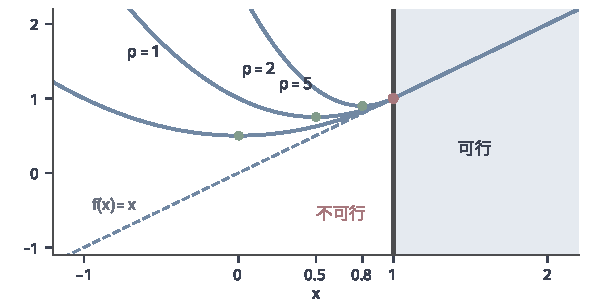
\includegraphics[width=100mm]{figures/05-optimization/06-constrained-optimization/matplotlib/pm-quad-1d/figure.pdf}
  \caption{一维例的二次罚函数，$\rho=1,2,5$。蓝色实线是$Q_\rho$，蓝色虚线是原目标$f(x)=x$，浅蓝区域是可行集，深灰竖线是约束边界。绿点是$Q_\rho$的最小点$x_\rho=1-1/\rho$，红点是原问题的解。有限的$\rho$下最小点总在边界左侧。}
  \label{fig:pm-quad-1d}
\end{BookInlineFigure}

\paragraph{力的平衡}
为什么有限的$\rho$总留下违规？把驻点方程$\rho(1-x_\rho)=1$读成力的平衡。目标以大小为$1$的力把$x$往左拉，罚项像一根劲度为$\rho$的弹簧往右推。弹簧必须被拉长才有力，要平衡$1$的力就得拉长$1/\rho$。弹簧越硬，拉长越少，但只要力不为零，拉长量就不为零。

这个力的大小$\rho(1-x_\rho)=1$恰好是最优乘子$\lambda^\star=1$。第~\ref{chap:constrained-optimality}章说过，乘子度量约束对目标的反作用力。这里违规量乘罚参数等于乘子，并不是一维例的巧合，后面会看到它的一般形式。类比也有失效的地方：真实的弹簧两边都有力，而不等式的罚项只在违规一侧起作用。

\begin{example}[二元例的二次罚]
\label{ex:pm-quadratic-running}
对式~\eqref{eq:pm-running}，罚函数是
\[
 Q_\rho(\bm{x})=\frac12x_1^2+\frac32x_2^2+\frac\rho2(x_1+x_2-4)^2 .
\]
令梯度为零，得到两个线性方程：
\[
 (1+\rho)x_1+\rho x_2=4\rho,\qquad \rho x_1+(3+\rho)x_2=4\rho .
\]
两式相减得$x_1=3x_2$。代回第二式，解出
\begin{equation}
 x_2(\rho)=\frac{4\rho}{3+4\rho},\qquad x_1(\rho)=\frac{12\rho}{3+4\rho}.
 \label{eq:pm-running-penalty-solution}
\end{equation}
由此算出约束残差
\begin{equation}
 h(\bm{x}(\rho))=-\frac{12}{3+4\rho}.
 \label{eq:pm-running-penalty-residual}
\end{equation}
它在$\rho\to\infty$时以$1/\rho$的速度趋于零，而$\rho h(\bm{x}(\rho))$趋于$-3$，正是$\nu^\star$。
\end{example}

图~\ref{fig:pm-penalty-contours}是同一个例子的二维图景。深灰直线是约束，绿点是$Q_\rho$的最小点。$\rho$增大时等高线沿直线方向被拉长，绿点向红点靠近。

\begin{BookInlineFigure}
  \centering
  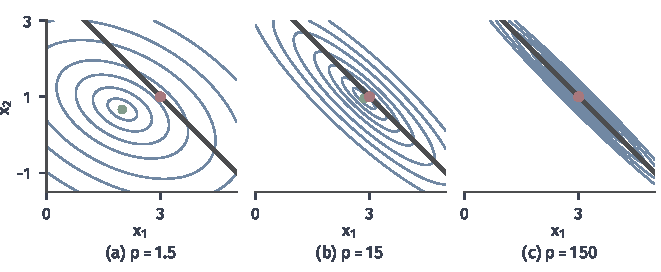
\includegraphics[width=112mm]{figures/05-optimization/06-constrained-optimization/matplotlib/pm-penalty-contours/figure.pdf}
  \caption{二元例中$Q_\rho$的等高线（蓝）。深灰直线是约束$x_1+x_2=4$，绿点是$Q_\rho$的最小点，红点是原问题的解$(3,1)$。$\rho$增大时最小点靠近解，等高线同时变成贴着约束的狭长椭圆。}
  \label{fig:pm-penalty-contours}
\end{BookInlineFigure}

\subsection{罚参数的更新}
\label{sec:pm-rho-update}

\paragraph{主要思想}
式~\eqref{eq:pm-running-penalty-residual}提示一开始就把$\rho$取得很大，一次解完。这样做的问题在于，$\rho$大的罚问题很难解，本节后面会算出来。如果从不好的初值开始，内层算法可能花大量步数才能进入解的附近。

合理的做法是沿着$\rho$的路径走。先取较小的$\rho$，解一个容易的问题；再放大$\rho$，以上一轮的解作为初值。$\rho$只放大有限倍时，新解离旧解不远，这叫\term{热启动}（warm start）。外层循环的结构如图~\ref{fig:pm-outer-loop}所示。

\begin{BookInlineFigure}
  \centering
  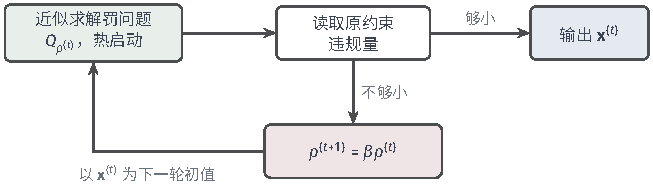
\includegraphics[width=110mm]{figures/05-optimization/06-constrained-optimization/tikz/pm-outer-loop/figure.pdf}
  \caption{二次惩罚法的外层循环。绿框是内层的无约束求解，蓝框是输出；判断依据是原约束的违规量，而不是罚目标的大小。只有违规量不够小时才放大罚参数（红框）。}
  \label{fig:pm-outer-loop}
\end{BookInlineFigure}

这里有两个容差，分工不同。内层容差$\omega^{(t)}$控制$\lVert\nabla Q_{\rho^{(t)}}(\bm{x}^{(t)})\rVert_2$，说明这一轮的罚问题解得多准。外层容差$\varepsilon$控制原约束的违规量，说明原问题的可行性够不够。内层梯度很小，只说明罚问题解好了，不能据此宣布原问题已解。

放大规则取固定倍数$\beta>1$，并记录乘子估计：
\begin{equation}
 \rho^{(t+1)}=\beta\rho^{(t)},\qquad
 \nu_j^{(t)}=\rho^{(t)}h_j(\bm{x}^{(t)}),\qquad
 \lambda_i^{(t)}=\rho^{(t)}[g_i(\bm{x}^{(t)})]_+ .
 \label{eq:pm-penalty-update}
\end{equation}
这组估计的来历可以从式~\eqref{eq:pm-quadratic-gradient}读出：把它们代入，$\nabla Q_{\rho}$恰好是Lagrange函数对$\bm{x}$的梯度。内层求解到梯度为零，就等于Lagrange驻定条件在这组估计下成立。

\paragraph{计算过程}
以二元例为例，内层用步长为$1/L$的梯度法，其中$L$是$\nabla^2Q_\rho$的最大特征值。

\needspace{6\baselineskip}
\paragraph{变量}
\begin{itemize}
 \item $\bm{x}^{(t)}\in\mathbb{R}^n$：第$t$轮罚问题的近似解。例中$n=2$。
 \item $\rho^{(t)}>0$：罚参数，放大倍数为$\beta>1$。
 \item $\varepsilon$、$\omega^{(t)}$：外层违规容差、内层梯度容差。
\end{itemize}

\paragraph{初始化}
取初值$\bm{x}^{(-1)}$、$\rho^{(0)}>0$和$\beta$。例中$\bm{x}^{(-1)}=(0,0)$，$\rho^{(0)}=1.5$，$\beta=10$，外层容差$\varepsilon=0.05$，内层容差取常数$\omega^{(t)}=10^{-3}$。

\needspace{6\baselineskip}
\paragraph{每轮更新}
\begin{enumerate}
 \item 从$\bm{x}^{(t-1)}$出发近似最小化$Q_{\rho^{(t)}}$，直到梯度范数不超过$\omega^{(t)}$。例中第一轮用了$21$个梯度步，结果接近式~\eqref{eq:pm-running-penalty-solution}的精确解，以下数值用精确解给出：
 \[
  \bm{x}^{(0)}=\Bigl(2,\ \frac23\Bigr).
 \]

 \item 计算违规量。例中第一轮
 \[
  h(\bm{x}^{(0)})=-\frac43,\qquad \lvert h(\bm{x}^{(0)})\rvert>\varepsilon .
 \]
 \item 若违规量不超过$\varepsilon$，结束；否则由式~\eqref{eq:pm-penalty-update}放大罚参数并记录乘子估计。例中第一轮
 \[
  \rho^{(1)}=15,\qquad \nu^{(0)}=1.5\times\Bigl(-\frac43\Bigr)=-2 .
 \]
\end{enumerate}
例中第二轮从$\bm{x}^{(0)}$热启动，用了$107$个梯度步，得到
\[
 \bm{x}^{(1)}=\Bigl(\frac{20}{7},\ \frac{20}{21}\Bigr),\qquad
 h(\bm{x}^{(1)})=-\frac{4}{21}\approx-0.190 .
\]
乘子估计是$\nu^{(1)}=-\tfrac{20}{7}\approx-2.857$。
违规量仍大于$0.05$，于是$\rho^{(2)}=150$。第三轮用了$725$个梯度步，得到
\[
 \bm{x}^{(2)}=\Bigl(\frac{200}{67},\ \frac{200}{201}\Bigr),\qquad
 h(\bm{x}^{(2)})=-\frac{4}{201}\approx-0.020 .
\]
乘子估计是$\nu^{(2)}=-\tfrac{200}{67}\approx-2.985$。

结束条件是违规量不超过$\varepsilon$，例中在第三轮满足。最终得到$\bm{x}^{(2)}\approx(2.985,0.995)$，目标值$f(\bm{x}^{(2)})\approx5.940$，略低于$f^\star=6$，这是因为点还不可行。三轮的梯度步数依次是$21$、$107$、$725$，几乎全部花在最后一轮上。步数为什么增长这么快，正是下一小节要回答的。

\subsection{极限与病态}
\label{sec:pm-limit}

这一小节回答两个问题：$\rho\to\infty$时迭代点到底趋于什么，以及这条路有多贵。

\paragraph{全局解的极限}
先看最理想的情形，每一轮都得到罚问题的全局最小点。此时可以把罚目标与任意一个可行点比较，这个比较给出全部结论。

\begin{theorem}[二次惩罚法的全局极限]
\label{thm:pm-quadratic-limit}
设$f$、$g_i$、$h_j$在$\mathbb{R}^n$上连续，可行集$\bm{C}$非空，且$f$在$\mathbb{R}^n$上有下界$f_{\mathrm{low}}$。设$\rho^{(t)}\to\infty$，每个$\bm{x}^{(t)}$都是$Q_{\rho^{(t)}}$的全局最小点。记
\begin{equation}
 v(\bm{x})=\sum_{i=1}^m[g_i(\bm{x})]_+^2+\sum_{j=1}^ph_j(\bm{x})^2 .
 \label{eq:pm-violation-square}
\end{equation}
则对任一可行点$\bar{\bm{x}}\in\bm{C}$，有
\begin{equation}
 v(\bm{x}^{(t)})\leq\frac{2\bigl(f(\bar{\bm{x}})-f_{\mathrm{low}}\bigr)}{\rho^{(t)}},
 \label{eq:pm-quadratic-violation-bound}
\end{equation}
并且$\{\bm{x}^{(t)}\}$的每个聚点都是原问题的全局最优解。
\end{theorem}

\begin{proof}
可行点上罚项为零，$Q_{\rho^{(t)}}(\bar{\bm{x}})=f(\bar{\bm{x}})$。$\bm{x}^{(t)}$是全局最小点，所以
\[
 f(\bm{x}^{(t)})+\frac{\rho^{(t)}}{2}v(\bm{x}^{(t)})\leq f(\bar{\bm{x}}).
\]
左边第一项用$f_{\mathrm{low}}$放缩，整理即得式~\eqref{eq:pm-quadratic-violation-bound}。

设$\hat{\bm{x}}$是一个聚点，子列收敛到它。$v$连续，而式~\eqref{eq:pm-quadratic-violation-bound}的右边趋于零，所以$v(\hat{\bm{x}})=0$，即$\hat{\bm{x}}$可行。

上面的不等式中罚项非负，去掉后得到
\[
 f(\bm{x}^{(t)})\leq f(\bar{\bm{x}}).
\]
沿子列取极限，由$f$连续得$f(\hat{\bm{x}})\leq f(\bar{\bm{x}})$。$\bar{\bm{x}}$是任取的可行点，所以$\hat{\bm{x}}$全局最优。
\end{proof}

各条件的作用分得很清楚。可行集非空提供了比较点$\bar{\bm{x}}$。下界把违规量和$\rho$联系起来。连续性保证极限可行，并让目标比较传到极限。“全局最小点”是证明的关键一步，局部解不能和远处的可行点比较。定理也不保证聚点存在：序列可能跑向无穷远，要排除这种情形，还需要类似水平集有界的条件。

去掉下界会怎样？考虑$\min x^3$，$x\geq0$，解是$x^\star=0$。罚函数在$x<0$时等于$x^3+\tfrac\rho2x^2$，$x\to-\infty$时趋于$-\infty$，所以对任何$\rho$都没有全局最小点。图~\ref{fig:pm-failures}(a)画出了这种情形：$x=0$附近有一个局部的谷，越过左侧的小山就一路下降。原问题完全正常，罚问题却无下界。

\paragraph{近似解的极限}
实际算法只能给出梯度小的点，通常连局部最小都不能保证。这时比较可行点的论证失效，能说的话变少，并且要多加条件。下面只写等式约束，记$\bm{h}(\bm{x})=(h_1(\bm{x}),\ldots,h_p(\bm{x}))$，$\bm{J}(\bm{x})\in\mathbb{R}^{p\times n}$是它的Jacobian矩阵。

\begin{theorem}[近似驻点的极限]
\label{thm:pm-quadratic-approximate}
设$f,h_j$连续可微，$\rho^{(t)}\to\infty$，并且
\begin{equation}
 \lVert\nabla Q_{\rho^{(t)}}(\bm{x}^{(t)})\rVert_2\leq\omega^{(t)}\to0 .
 \label{eq:pm-inner-accuracy}
\end{equation}
设$\hat{\bm{x}}$是$\{\bm{x}^{(t)}\}$的聚点，则$\hat{\bm{x}}$是$\tfrac12\lVert\bm{h}\rVert_2^2$的驻点。若进一步$\hat{\bm{x}}$可行且$\bm{J}(\hat{\bm{x}})$行满秩，则沿收敛到$\hat{\bm{x}}$的子列有
\begin{equation}
 \rho^{(t)}\bm{h}(\bm{x}^{(t)})\to\hat{\bm{\nu}},\qquad
 \nabla f(\hat{\bm{x}})+\bm{J}(\hat{\bm{x}})^\top\hat{\bm{\nu}}=\bm{0},
 \label{eq:pm-multiplier-limit}
\end{equation}
即$(\hat{\bm{x}},\hat{\bm{\nu}})$满足KKT条件。
\end{theorem}

\begin{proof}
记$\bm{e}^{(t)}=\nabla Q_{\rho^{(t)}}(\bm{x}^{(t)})$，$\bm{e}^{(t)}\to\bm{0}$。为简化写法，下面的量都沿子列取，并省略$\bm{x}^{(t)}$的自变量。由梯度公式，
\[
 \nabla f+\rho^{(t)}\bm{J}^\top\bm{h}=\bm{e}^{(t)}.
\]
两边除以$\rho^{(t)}$，得到
\[
 \bm{J}^\top\bm{h}=\frac{\bm{e}^{(t)}-\nabla f}{\rho^{(t)}}.
\]
右边的分子有界，分母趋于无穷，取极限得
\[
 \bm{J}(\hat{\bm{x}})^\top\bm{h}(\hat{\bm{x}})=\bm{0}.
\]
左边正是$\tfrac12\lVert\bm{h}\rVert_2^2$的梯度，第一个结论成立。

再设$\hat{\bm{x}}$可行且$\bm{J}(\hat{\bm{x}})$行满秩。$\bm{J}\bm{J}^\top$连续且极限可逆，所以$t$足够大时可逆。用$\bm{J}$左乘第一个等式再求逆，解出
\[
 \rho^{(t)}\bm{h}=(\bm{J}\bm{J}^\top)^{-1}\bm{J}\bigl(\bm{e}^{(t)}-\nabla f\bigr).
\]
右边收敛，记极限为$\hat{\bm{\nu}}$。把$\rho^{(t)}\bm{h}\to\hat{\bm{\nu}}$代回第一个等式取极限，即得式~\eqref{eq:pm-multiplier-limit}。
\end{proof}

这个定理有两点值得注意。第一，$\hat{\bm{x}}$完全可能不可行，它只是约束残差平方的驻点。第二，定理的结论停在KKT点，和全局最优还差得远。

下面的例子显示第一点确实会发生。取
\[
 \min_x\ \frac12x^2\qquad\text{s.t.}\qquad h(x)=x^3-3x+3=0 .
\]
三次方程只有一个实根$x^\star\approx-2.104$，这也是唯一的可行点。$h$在$x=1$处有局部极小值$h(1)=1$，所以$\tfrac12h^2$在这里有一个不可行的局部谷。图~\ref{fig:pm-failures}(b)中绿点是$Q_3$在这个谷里的局部最小点。

取$\rho=10$和$\rho=100$，用二分法解$Q_\rho'(x)=0$，得到谷中的驻点分别是
\[
 x_{10}\approx0.9835,\qquad x_{100}\approx0.9983 .
\]
这两个点上$Q_\rho$的梯度为零，$h$却约等于$1$。放大$\rho$只会让点更靠近$x=1$，乘子估计$\rho h$随之发散。乘子估计发散正是不可行极限的常见信号。

\begin{BookInlineFigure}
  \centering
  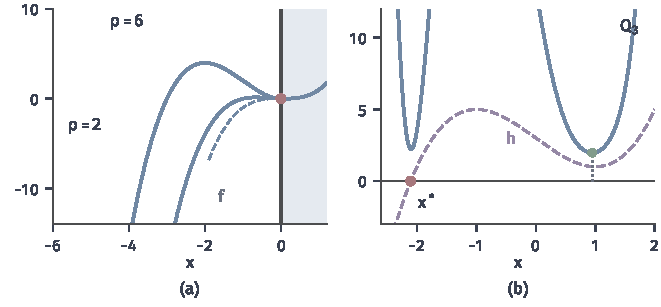
\includegraphics[width=112mm]{figures/05-optimization/06-constrained-optimization/matplotlib/pm-failures/figure.pdf}
  \caption{二次惩罚法的两种失败。(a)$\min x^3$，$x\geq0$：蓝色实线是$\rho=2,6$的罚函数，虚线是$f$的一段，浅蓝区域可行，红点是解；$x\to-\infty$时罚函数无下界。(b)$\min\tfrac12x^2$，$h(x)=x^3-3x+3=0$：紫色虚线是$h$，蓝线是$Q_3$，红点是唯一的可行点，绿点是不可行的局部最小点。}
  \label{fig:pm-failures}
\end{BookInlineFigure}

\paragraph{法向曲率的增长}
剩下的问题是代价。对等式约束的罚函数求二阶导，得到
\begin{equation}
 \nabla^2Q_\rho=\nabla^2f+\rho\sum_{j=1}^ph_j\nabla^2h_j+\rho\bm{J}^\top\bm{J}.
 \label{eq:pm-penalty-hessian}
\end{equation}
由定理~\ref{thm:pm-quadratic-approximate}，$\rho h_j$在解附近接近有限的乘子，前两项之和接近Lagrange函数的Hessian，大小不随$\rho$增长。第三项却正比于$\rho$，它只在$\bm{J}$的行空间里起作用，也就是约束的法方向上。

线性约束的二次目标可以把这件事算清楚。设目标和约束分别是
\[
 f(\bm{x})=\frac12\bm{x}^\top\bm{G}\bm{x}-\bm{d}^\top\bm{x},\qquad\bm{h}(\bm{x})=\bm{A}\bm{x}-\bm{b},
\]
其中$\bm{A}\in\mathbb{R}^{p\times n}$，$p<n$，$\bm{G}$半正定。此时$\nabla^2Q_\rho=\bm{G}+\rho\bm{A}^\top\bm{A}$不依赖$\bm{x}$。

\begin{lemma}[罚函数Hessian的条件数]
\label{lem:pm-penalty-condition}
设$\bm{A}\neq\bm{0}$，$\bm{Z}$的列是$\operatorname{null}(\bm{A})$的一组标准正交基，矩阵$\bm{Z}^\top\bm{G}\bm{Z}$正定，$\sigma_{\max}(\bm{A})$是$\bm{A}$的最大奇异值。记$\bm{H}_\rho=\bm{G}+\rho\bm{A}^\top\bm{A}$。当$\bm{H}_\rho$正定时，有
\begin{equation}
 \lambda_{\max}(\bm{H}_\rho)\geq\rho\,\sigma_{\max}(\bm{A})^2,\qquad
 \lambda_{\min}(\bm{H}_\rho)\leq\lambda_{\min}(\bm{Z}^\top\bm{G}\bm{Z}),
 \label{eq:pm-penalty-eigen-bounds}
\end{equation}
于是条件数满足
\begin{equation}
 \kappa(\bm{H}_\rho)\geq\frac{\rho\,\sigma_{\max}(\bm{A})^2}{\lambda_{\min}(\bm{Z}^\top\bm{G}\bm{Z})}.
 \label{eq:pm-penalty-condition}
\end{equation}
\end{lemma}

\begin{proof}
两个界都来自Rayleigh商。设$\bm{u}$是$\bm{A}$对应最大奇异值的单位右奇异向量。由$\bm{G}$半正定，
\[
 \lambda_{\max}(\bm{H}_\rho)\geq\bm{u}^\top\bm{H}_\rho\bm{u}\geq\rho\lVert\bm{A}\bm{u}\rVert_2^2=\rho\,\sigma_{\max}(\bm{A})^2 .
\]
再取单位向量$\bm{w}$，使它达到$\bm{Z}^\top\bm{G}\bm{Z}$的最小特征值，并令$\bm{y}=\bm{Z}\bm{w}$。$\bm{y}$是单位向量且$\bm{A}\bm{y}=\bm{0}$，所以罚项消失：
\[
 \lambda_{\min}(\bm{H}_\rho)\leq\bm{y}^\top\bm{H}_\rho\bm{y}=\bm{w}^\top\bm{Z}^\top\bm{G}\bm{Z}\bm{w}=\lambda_{\min}(\bm{Z}^\top\bm{G}\bm{Z}).
\]
两式相除，即得式~\eqref{eq:pm-penalty-condition}。
\end{proof}

几何上看，$\bm{H}_\rho$把空间分成两部分：沿约束的切方向，曲率不受$\rho$影响；沿法方向，曲率约正比于$\rho$。这就是图~\ref{fig:pm-penalty-contours}里等高线越来越狭长的原因。

二元例中$\bm{G}=\operatorname{diag}(1,3)$，$\bm{A}=(1,1)$，$\sigma_{\max}(\bm{A})^2=2$。切方向是单位向量$(1,-1)/\sqrt2$，切向曲率是
\[
 \bm{Z}^\top\bm{G}\bm{Z}=\frac{1+3}{2}=2 .
\]
下表给出$\bm{H}_\rho$的实际特征值，最小特征值逐渐接近切向曲率$2$，最大特征值约等于$2\rho$。

\begin{BookInlineTable}
  \centering
  \begin{tabular}{@{}rrrr@{}}
    \toprule
    $\rho$ & $\lambda_{\min}$ & $\lambda_{\max}$ & $\kappa$\\
    \midrule
    $1.5$ & $1.697$ & $5.303$ & $3.1$\\
    $15$ & $1.967$ & $32.03$ & $16.3$\\
    $150$ & $1.997$ & $302.0$ & $151.3$\\
    $1500$ & $2.000$ & $3002$ & $1501$\\
    \bottomrule
  \end{tabular}
  \caption{二元例中罚函数Hessian的特征值与条件数。}
  \label{tab:pm-penalty-condition}
\end{BookInlineTable}

图~\ref{fig:pm-conditioning}把精度和代价放在一起。(a)是违规量，$\rho$放大十倍，违规量缩小十倍。(b)是条件数和梯度步数，$\rho$放大十倍，条件数也放大十倍，每轮的梯度步数增长的倍数相近。

\begin{BookInlineFigure}
  \centering
  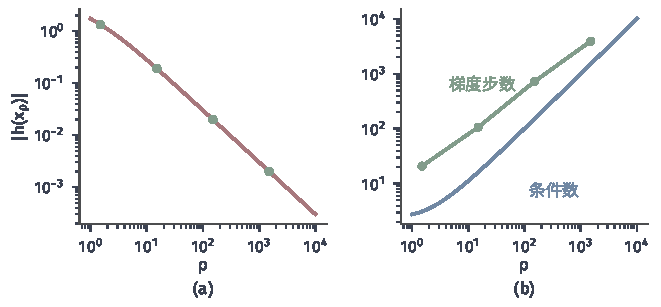
\includegraphics[width=112mm]{figures/05-optimization/06-constrained-optimization/matplotlib/pm-conditioning/figure.pdf}
  \caption{二元例中罚参数的收益与代价，双对数坐标。(a)精确罚解的违规量$12/(3+4\rho)$，绿点是$\rho=1.5,15,150,1500$。(b)蓝线是$\nabla^2Q_\rho$的条件数，绿线是热启动的梯度法（步长$1/L$，梯度容差$10^{-3}$）在各轮用的步数。}
  \label{fig:pm-conditioning}
\end{BookInlineFigure}

梯度法的困难可以直接看到。图~\ref{fig:pm-gd-penalty}从同一点出发各走$25$步。$\rho=1.5$时点很快到达最小点附近；$\rho=15$时第一步几乎只修正法向，点落到直线旁边，然后沿狭长山谷缓慢爬行，$25$步还没有走到。步长受最大曲率限制，只能取$1/L\approx1/(2\rho)$，切方向每步却只能修正很小一部分。

\begin{BookInlineFigure}
  \centering
  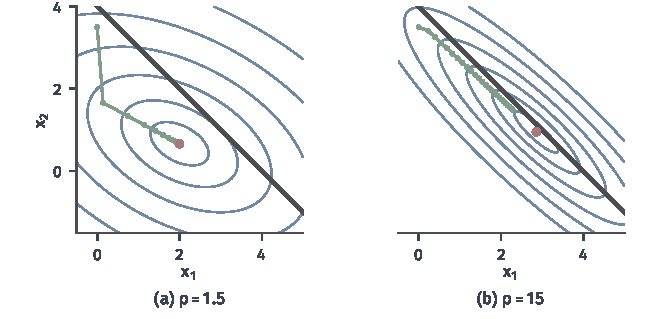
\includegraphics[width=112mm]{figures/05-optimization/06-constrained-optimization/matplotlib/pm-gd-penalty/figure.pdf}
  \caption{梯度法在$Q_\rho$上的路径，起点$(0,3.5)$，步长$1/L$，共$25$步。蓝线是$Q_\rho$的等高线，深灰直线是约束，绿色折线是迭代路径，红点是$Q_\rho$的最小点。(a)$\rho=1.5$，几步后接近最小点。(b)$\rho=15$，先快速到达山谷，再沿谷底缓慢前进。}
  \label{fig:pm-gd-penalty}
\end{BookInlineFigure}

病态是否致命，取决于内层用什么方法。Newton法不怕目标的简单伸缩，但线性方程组$\bm{H}_\rho\bm{d}=-\nabla Q_\rho$的系数矩阵本身条件数很差。引入$\bm{w}=\rho\bm{A}\bm{d}$，可以把它等价地写成
\begin{equation}
 \begin{pmatrix}\bm{G}&\bm{A}^\top\\\bm{A}&-\rho^{-1}\bm{I}\end{pmatrix}
 \begin{pmatrix}\bm{d}\\\bm{w}\end{pmatrix}
 =\begin{pmatrix}-\nabla Q_\rho\\\bm{0}\end{pmatrix}.
 \label{eq:pm-penalty-augmented-system}
\end{equation}
$\rho\to\infty$时这个系统趋于一个不含大数的KKT矩阵，数值上稳定得多。这个变换改善的是线性代数的数值误差，并不减少外层要解的问题个数。一阶方法没有这种办法。第~\ref{sec:pm-alm}节要给出另一条出路：不把$\rho$推向无穷。

\section{精确惩罚法}
\label{sec:pm-exact}

上一节的二次罚必须把$\rho$推向无穷，原因就在罚项本身：平方函数在零点的斜率是零。可行边界上，罚项完全没有回推的力，目标只要有一点斜率，点就会越过边界，直到弹簧被拉长。这就需要回答：换一种在边界上就有斜率的罚项，有限的$\rho$能否直接得到原问题的解？

\paragraph{一次罚函数}
把平方换成绝对值和正部本身，在零点就有了尖角：

\begin{definition}[一次罚函数]
\label{def:pm-exact-penalty}
对问题~\eqref{eq:pm-problem}和$\rho>0$，记总违规量
\begin{equation}
 V(\bm{x})=\sum_{i=1}^m[g_i(\bm{x})]_++\sum_{j=1}^p\lvert h_j(\bm{x})\rvert ,
 \label{eq:pm-total-violation}
\end{equation}
称
\begin{equation}
 E_\rho(\bm{x})=f(\bm{x})+\rho V(\bm{x})
 \label{eq:pm-exact-penalty}
\end{equation}
为\term{一次罚函数}（$\ell_1$ penalty function）。若存在有限的$\rho$，使$E_\rho$的最小点就是原问题的最小点，就称这个罚函数是\term{精确罚函数}（exact penalty function）。
\end{definition}

“精确”说的是两个问题的解之间的对应关系。它并不表示数值上已经把子问题解到了机器精度，也不表示算法可以一步得到解。

\begin{example}[一维例的一次罚]
\label{ex:pm-exact-one-dim}
式~\eqref{eq:pm-one-dim}的一次罚函数是
\[
 E_\rho(x)=x+\rho[1-x]_+ .
\]
$x>1$时斜率是$1$，$x<1$时斜率是$1-\rho$。结果按$\rho$分成三种情形：
\begin{itemize}
 \item $\rho<1$时，$x<1$的一侧斜率为正，$x\to-\infty$时$E_\rho\to-\infty$，没有最小点；
 \item $\rho=1$时，$x\leq1$的整条射线上$E_\rho\equiv1$，最小点集合比原问题的解大；
 \item $\rho>1$时，$E_\rho$在$x=1$处由负斜率转为正斜率，$x=1$是唯一最小点。
\end{itemize}
门槛恰好是$\lambda^\star=1$。
\end{example}

图~\ref{fig:pm-exact-1d}(a)画出这三种情形。尖角的作用从图上一眼可见：只要左边的斜率足够陡，最低点就被“钉”在尖角上，不需要$\rho$继续增大。这和一元绝对值函数的最小点停在零点，是同一种机制。

\begin{BookInlineFigure}
  \centering
  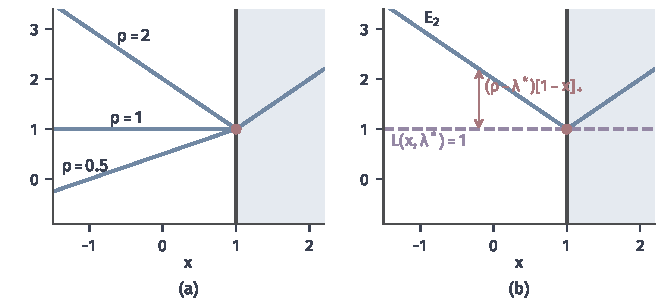
\includegraphics[width=112mm]{figures/05-optimization/06-constrained-optimization/matplotlib/pm-exact-1d/figure.pdf}
  \caption{一维例的一次罚函数。浅蓝区域可行，深灰竖线是约束边界，红点是解$x^\star=1$。(a)蓝线是$\rho=0.5,1,2$的$E_\rho$：$\rho<1$无下界，$\rho=1$左侧水平，$\rho>1$最小点就是$x^\star$。(b)蓝线是$E_2$，紫色虚线是Lagrange函数$\mathcal{L}(x,\lambda^\star)\equiv1$，$E_2$在它上方，红色箭头是两者之差。}
  \label{fig:pm-exact-1d}
\end{BookInlineFigure}

\paragraph{二元例的比较}
式~\eqref{eq:pm-running}的一次罚函数是
\[
 E_\rho(\bm{x})=\frac12x_1^2+\frac32x_2^2+\rho\lvert x_1+x_2-4\rvert .
\]
最优性条件是存在$\xi\in\partial\lvert\cdot\rvert(h(\bm{x}))$，使$\bm{x}$满足
\[
 x_1+\rho\xi=0,\qquad 3x_2+\rho\xi=0 .
\]
其中$\xi=\operatorname{sign}(h)$（当$h\neq0$），$\xi\in[-1,1]$（当$h=0$）。先假设解落在$h<0$的一侧，此时$\xi=-1$，解出
\[
 \bm{x}=\rho\Bigl(1,\ \frac13\Bigr).
\]
$h<0$要求$\tfrac43\rho-4<0$，即$\rho<3$。当$\rho\geq3$时，取$h=0$，也就是$\bm{x}=(3,1)$，由第一个方程得
\[
 \xi=-\frac{3}{\rho}\in[-1,0).
\]
所以$\rho\geq3$时解就是$\bm{x}^\star$，门槛是$\lvert\nu^\star\rvert=3$。

图~\ref{fig:pm-exact-path}把两种罚放在同一张图里。二次罚的$x_1(\rho)$永远在逼近$3$而到不了；一次罚先沿直线上升，在$\rho=3$处到达$3$，此后不再变化，违规量恰好为零。代价是$\rho<3$时一次罚的违规量可能更大，并且$E_\rho$在解处不可微。

\begin{BookInlineFigure}
  \centering
  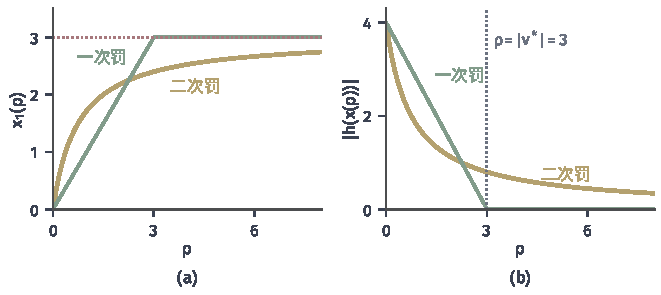
\includegraphics[width=112mm]{figures/05-optimization/06-constrained-optimization/matplotlib/pm-exact-path/figure.pdf}
  \caption{二元例中两种罚函数的解随$\rho$变化。黄线是二次罚，绿线是一次罚，(a)中红色点线是$x_1^\star=3$。(a)第一个坐标：二次罚只能渐近，一次罚在$\rho=3$到达并停住。(b)违规量：一次罚在$\rho\geq3$时恰为零，门槛等于$\lvert\nu^\star\rvert$。}
  \label{fig:pm-exact-path}
\end{BookInlineFigure}

\begin{BookInlineTable}
  \centering
  \begin{tabular}{@{}lll@{}}
    \toprule
     & 二次罚$Q_\rho$ & 一次罚$E_\rho$\\
    \midrule
    边界上的斜率 & 零 & 非零\\
    有限$\rho$的解 & 一般不可行 & 超过门槛后可行\\
    光滑性 & 一阶连续可微 & 边界上不可微\\
    $\rho$的取法 & 必须趋于无穷 & 只需超过乘子门槛\\
    内层困难 & 法向曲率增长 & 解处有尖角\\
    \bottomrule
  \end{tabular}
  \caption{二次罚与一次罚的对照。二次罚以病态换取光滑，一次罚以不可微换取有限的罚参数。}
  \label{tab:pm-penalty-contrast}
\end{BookInlineTable}

\subsection{精确性的条件}
\label{sec:pm-exact-conditions}

门槛和乘子的关系不是例子的巧合。下面要把它写成定理，并分清全局和局部两个层次。

\paragraph{全局精确性}
回忆第~\ref{chap:duality}章的记号。Lagrange函数是
\[
 \mathcal{L}(\bm{x},\bm{\lambda},\bm{\nu})=f(\bm{x})+\sum_{i=1}^m\lambda_ig_i(\bm{x})+\sum_{j=1}^p\nu_jh_j(\bm{x}),
\]
对偶函数$q$是$\mathcal{L}$对$\bm{x}$的下确界。弱对偶说$\bm{\lambda}\geq\bm{0}$时$q(\bm{\lambda},\bm{\nu})\leq f^\star$；强对偶说存在$(\bm{\lambda}^\star,\bm{\nu}^\star)$使等号成立。这个下界和一次罚函数放在一起，就是图~\ref{fig:pm-exact-1d}(b)的画面：$\mathcal{L}(x,\lambda^\star)$是整条水平线，$E_\rho$处处在它上方。

\begin{theorem}[一次罚的全局精确性]
\label{thm:pm-exact-global}
设原问题的最优解$\bm{x}^\star$存在，对偶问题的最优解$(\bm{\lambda}^\star,\bm{\nu}^\star)$存在，且强对偶成立，$q(\bm{\lambda}^\star,\bm{\nu}^\star)=f^\star$。若
\begin{equation}
 \rho>\max\Bigl\{\max_i\lambda_i^\star,\ \max_j\lvert\nu_j^\star\rvert\Bigr\},
 \label{eq:pm-exact-threshold}
\end{equation}
则$E_\rho$的全局最小点集合恰好等于原问题的全局最优解集合，且对所有$\bm{x}$有
\begin{equation}
 E_\rho(\bm{x})\geq f^\star+\delta V(\bm{x}),
 \label{eq:pm-exact-lower-bound}
\end{equation}
其中$\delta>0$是$\rho$与门槛之差。
\end{theorem}

\begin{proof}
记门槛为$\rho_0$，$\delta=\rho-\rho_0>0$。先建立式~\eqref{eq:pm-exact-lower-bound}。由$\lambda_i^\star\geq0$和$g_i\leq[g_i]_+$，有
\[
 \lambda_i^\star g_i(\bm{x})\leq\lambda_i^\star[g_i(\bm{x})]_+\leq\rho_0[g_i(\bm{x})]_+ .
\]
对等式项同样有
\[
 \nu_j^\star h_j(\bm{x})\leq\lvert\nu_j^\star\rvert\lvert h_j(\bm{x})\rvert\leq\rho_0\lvert h_j(\bm{x})\rvert .
\]
把这些不等式对$i,j$求和，得到
\[
 \sum_i\lambda_i^\star g_i(\bm{x})+\sum_j\nu_j^\star h_j(\bm{x})\leq\rho_0V(\bm{x}).
\]

于是
\[
 \begin{aligned}
 E_\rho(\bm{x})&=f(\bm{x})+\rho_0V(\bm{x})+\delta V(\bm{x})\\
 &\geq\mathcal{L}(\bm{x},\bm{\lambda}^\star,\bm{\nu}^\star)+\delta V(\bm{x})\\
 &\geq q(\bm{\lambda}^\star,\bm{\nu}^\star)+\delta V(\bm{x}).
 \end{aligned}
\]
由强对偶，最后一式等于$f^\star+\delta V(\bm{x})$，这就是式~\eqref{eq:pm-exact-lower-bound}。

再看最小点集合。任一原问题最优解$\bm{x}^\star$满足$V(\bm{x}^\star)=0$，$E_\rho(\bm{x}^\star)=f^\star$，由下界知它是$E_\rho$的全局最小点，且$E_\rho$的最小值是$f^\star$。

反过来，设$\bar{\bm{x}}$是$E_\rho$的全局最小点，则$E_\rho(\bar{\bm{x}})=f^\star$。代入下界得$\delta V(\bar{\bm{x}})\leq0$，所以$V(\bar{\bm{x}})=0$，$\bar{\bm{x}}$可行。此时$f(\bar{\bm{x}})=E_\rho(\bar{\bm{x}})=f^\star$，它是原问题的最优解。
\end{proof}

式~\eqref{eq:pm-exact-threshold}中的门槛用的是最大绝对分量，因为总违规量是$\ell_1$形式，两者互为对偶范数。门槛可以按任一组最优乘子计算，最优乘子不唯一时，取能使门槛最小的一组。

证明里没有用到凸性，全部负担都在强对偶上。对一般的非凸问题，强对偶很少成立，所以全局精确性主要是凸问题的结论；第~\ref{chap:duality}章给出的Slater条件是常用的充分条件。

严格不等号也不能省。一维例中$\rho=1$恰好等于门槛，$E_1$的最小点是整条射线$(-\infty,1]$，原问题的解只是其中一点。此时$\delta=0$，下界~\eqref{eq:pm-exact-lower-bound}里违规量的系数消失，最后一步推不出可行。

\paragraph{对偶解不存在时}
去掉“对偶最优解存在”，结论会彻底失败。考虑
\[
 \min_x\ x\qquad\text{s.t.}\qquad x^2\leq0 .
\]
可行集只有$\{0\}$，$x^\star=0$。这是凸问题，$q(\lambda)=-1/(4\lambda)$，$\lambda\to\infty$时趋于$0=f^\star$，但上确界取不到，不存在有限的最优乘子。它的一次罚是$E_\rho(x)=x+\rho x^2$，唯一最小点是
\[
 x_\rho=-\frac{1}{2\rho}\neq0 .
\]
对每个有限的$\rho$，最小点都不可行，$\rho$必须趋于无穷。这里约束的梯度在解处是零，违规量$x^2$在解处光滑，根本没有尖角。可见一次罚的尖角要靠约束的梯度才能起作用。

\paragraph{局部精确性}
非凸问题用不上强对偶，可以只问局部：$\bm{x}^\star$是否是$E_\rho$的局部最小点。局部分析有两条路线。一条看约束集的几何，要求违规量控制到可行集的距离；另一条看KKT条件和曲率。

第一条路线的条件是\term{局部误差界}（local error bound）：存在$\tau>0$和$\bm{x}^\star$的邻域，使邻域内的$\bm{x}$满足
\begin{equation}
 \operatorname{dist}(\bm{x},\bm{C})\leq\tau V(\bm{x}).
 \label{eq:pm-error-bound}
\end{equation}
它的意思是，违规量小就真的离可行集近，不会出现违规量几乎为零、点却还很远的情况。线性约束时误差界在整个空间成立，这是Hoffman界。对光滑约束，它在Mangasarian--Fromovitz约束资格下成立，证明需要用到非线性系统的度量正则性，篇幅较长，这里只使用结论。

第二条路线要用到二阶条件。在KKT点$(\bm{x}^\star,\bm{\lambda}^\star,\bm{\nu}^\star)$处，临界方向$\bm{d}$满足
\begin{equation}
 \nabla h_j(\bm{x}^\star)^\top\bm{d}=0,\qquad
 \begin{cases}
 \nabla g_i(\bm{x}^\star)^\top\bm{d}=0, & g_i(\bm{x}^\star)=0,\ \lambda_i^\star>0,\\
 \nabla g_i(\bm{x}^\star)^\top\bm{d}\leq0, & g_i(\bm{x}^\star)=0,\ \lambda_i^\star=0.
 \end{cases}
 \label{eq:pm-critical-cone}
\end{equation}
二阶充分条件要求Lagrange函数在KKT点处的Hessian沿每个非零临界方向$\bm{d}$都有正曲率：
\[
 \bm{d}^\top\nabla^2_{\bm{x}\bm{x}}\mathcal{L}(\bm{x}^\star,\bm{\lambda}^\star,\bm{\nu}^\star)\bm{d}>0 .
\]
它的含义第~\ref{chap:constrained-optimality}章已经建立。

\begin{theorem}[一次罚的局部精确性]
\label{thm:pm-exact-local}
设$\bm{x}^\star$是可行点。
\begin{enumerate}
 \item 设$\bm{C}$是闭集，$\bm{x}^\star$是$f$在$\bm{C}$上的局部最小点，$f$在$\bm{x}^\star$的邻域内$G$-Lipschitz，且局部误差界~\eqref{eq:pm-error-bound}成立。若$\rho>G\tau$，则$\bm{x}^\star$是$E_\rho$的局部最小点。
 \item 设$f,g_i,h_j$二阶连续可微，$(\bm{x}^\star,\bm{\lambda}^\star,\bm{\nu}^\star)$是KKT点并满足二阶充分条件。若$\rho$满足式~\eqref{eq:pm-exact-threshold}，则$\bm{x}^\star$是$E_\rho$的严格局部最小点。
\end{enumerate}
\end{theorem}

\begin{proof}
先证第一部分。取充分小的$r>0$，使$\lVert\bm{x}-\bm{x}^\star\rVert_2\leq r$时误差界成立，并使$\bm{x}^\star$在半径$2r$的球内是$f$在$\bm{C}$上的最小点，$f$在该球内$G$-Lipschitz。

任取这样的$\bm{x}$，设$\bm{y}$是$\bm{x}$在闭集$\bm{C}$上的一个最近点。$\bm{x}^\star$也在$\bm{C}$中，所以
\[
 \lVert\bm{x}-\bm{y}\rVert_2\leq\lVert\bm{x}-\bm{x}^\star\rVert_2\leq r .
\]
由三角不等式，$\bm{y}$在半径$2r$的球内。于是
\[
 f(\bm{x})\geq f(\bm{y})-G\lVert\bm{x}-\bm{y}\rVert_2\geq f(\bm{x}^\star)-G\tau V(\bm{x}).
\]
由此得
\[
 E_\rho(\bm{x})\geq f(\bm{x}^\star)+(\rho-G\tau)V(\bm{x})\geq E_\rho(\bm{x}^\star).
\]

再证第二部分，用反证法。设$\bm{x}^\star$不是严格局部最小点，则存在$\bm{x}^{(k)}\to\bm{x}^\star$，$\bm{x}^{(k)}\neq\bm{x}^\star$，$E_\rho(\bm{x}^{(k)})\leq f(\bm{x}^\star)$。记$\bm{d}^{(k)}=\bm{x}^{(k)}-\bm{x}^\star$，取子列使单位向量$\bm{d}^{(k)}/\lVert\bm{d}^{(k)}\rVert_2$收敛到$\bm{d}$。

记$\rho_0$为式~\eqref{eq:pm-exact-threshold}的右端，$\delta=\rho-\rho_0>0$，$[a]_-=\max\{-a,0\}$。对单个不等式约束，$a=g_i(\bm{x}^{(k)})$时有
\[
 \rho[a]_+-\lambda_i^\star a\geq\delta[a]_++\lambda_i^\star[a]_- .
\]
这个不等式分两种情形验证：$a>0$时左边等于$(\rho-\lambda_i^\star)a\geq\delta a$，$a\leq0$时左边等于$\lambda_i^\star\lvert a\rvert$。等式项类似，
\[
 \rho\lvert h_j\rvert-\nu_j^\star h_j\geq\delta\lvert h_j\rvert .
\]

把它们加起来，并用$\mathcal{L}^\star$表示乘子固定为$(\bm{\lambda}^\star,\bm{\nu}^\star)$的Lagrange函数，得到
\[
 E_\rho(\bm{x}^{(k)})\geq\mathcal{L}^\star(\bm{x}^{(k)})+\delta V(\bm{x}^{(k)})+\sum_i\lambda_i^\star[g_i(\bm{x}^{(k)})]_- .
\]
KKT条件给出$\mathcal{L}^\star(\bm{x}^\star)=f(\bm{x}^\star)$和$\nabla\mathcal{L}^\star(\bm{x}^\star)=\bm{0}$。作二阶展开，记$\bm{W}=\nabla^2\mathcal{L}^\star(\bm{x}^\star)$，则
\[
 \mathcal{L}^\star(\bm{x}^{(k)})=f(\bm{x}^\star)+\frac12(\bm{d}^{(k)})^\top\bm{W}\bm{d}^{(k)}+o(\lVert\bm{d}^{(k)}\rVert_2^2).
\]
结合$E_\rho(\bm{x}^{(k)})\leq f(\bm{x}^\star)$，得到
\[
 \delta V(\bm{x}^{(k)})+\sum_i\lambda_i^\star[g_i(\bm{x}^{(k)})]_-
 \leq-\frac12(\bm{d}^{(k)})^\top\bm{W}\bm{d}^{(k)}+o(\lVert\bm{d}^{(k)}\rVert_2^2).
\]

右边是$O(\lVert\bm{d}^{(k)}\rVert_2^2)$，所以左边每一项都是这个量级。展开$h_j(\bm{x}^{(k)})$，除以$\lVert\bm{d}^{(k)}\rVert_2$取极限，由$\lvert h_j\rvert=O(\lVert\bm{d}^{(k)}\rVert_2^2)$得$\nabla h_j(\bm{x}^\star)^\top\bm{d}=0$。对活动的$g_i$，$[g_i]_+=O(\lVert\bm{d}^{(k)}\rVert_2^2)$给出$\nabla g_i(\bm{x}^\star)^\top\bm{d}\leq0$；当$\lambda_i^\star>0$时，$[g_i]_-$也是这个量级，于是等号成立。所以$\bm{d}$是非零临界方向。

最后，上式左边非负。两边除以$\lVert\bm{d}^{(k)}\rVert_2^2$取极限，得到$\bm{d}^\top\bm{W}\bm{d}\leq0$，与二阶充分条件矛盾。
\end{proof}

两部分的结论都只说$\bm{x}^\star$附近的事。局部精确不等于全局精确，例如$\min-x^4$，约束$x=0$。此时$\nu^\star=0$，门槛是零，对任何$\rho>0$，$x=0$都是$E_\rho(x)=-x^4+\rho\lvert x\rvert$的严格局部最小点，而$x\to\infty$时$E_\rho\to-\infty$。

\subsection{非光滑罚问题的求解}
\label{sec:pm-exact-solve}

有了精确性，还要回答怎么解$E_\rho$。它的尖角恰好在解的位置上，光滑方法在这里不能直接使用。第~\ref{chap:nonsmooth-composite-optimization}章的工具可以逐一套用，但每种工具都要先核对问题的结构。

\paragraph{次梯度与最优性}
设$f$和$h_j$可微，问题是凸的。$0\in\partial E_\rho(\bm{x})$写开来，就是存在$\xi_j\in\partial\lvert\cdot\rvert(h_j(\bm{x}))$，使
\begin{equation}
 \nabla f(\bm{x})+\sum_{j=1}^p\rho\xi_j\nabla h_j(\bm{x})=\bm{0}.
 \label{eq:pm-exact-subgradient}
\end{equation}
和KKT的驻定方程比较，$\nu_j=\rho\xi_j$就是乘子估计。$\xi_j$落在$[-1,1]$内，$\lvert\nu_j\rvert\leq\rho$。如果解上某条约束的$\lvert\xi_j\rvert=1$且仍然违规，说明罚参数不够大，或者问题本身不可行。

次梯度法只需要这些$\xi_j$，但第~\ref{chap:nonsmooth-composite-optimization}章已经看到，步长固定时点会在尖角附近反复跳动，收敛很慢。图~\ref{fig:pm-exact-ista}里的黄线就是这种行为，它在约束直线两侧来回穿越，几乎每一步都不可行。

\paragraph{邻近梯度}
若把光滑部分$f$留给梯度步，把$\rho V$留给邻近步，就是第~\ref{chap:nonsmooth-composite-optimization}章的邻近梯度法。关键在于邻近映射能否算出。对二元例，设$\bm{a}=(1,1)$，$\tau=\alpha\rho$，要解的子问题是
\begin{equation}
 \bm{p}=\argmin_{\bm{x}}\ \frac12\lVert\bm{x}-\bm{v}\rVert_2^2+\tau\lvert\bm{a}^\top\bm{x}-4\rvert .
 \label{eq:pm-exact-prox}
\end{equation}
由最优性条件，存在$\lvert\cdot\rvert$在$\bm{a}^\top\bm{p}-4$处的次梯度$\xi$，使$\bm{p}=\bm{v}-\tau\xi\bm{a}$。两边与$\bm{a}$作内积，得到
\[
 \bm{a}^\top\bm{p}-4=\bm{a}^\top\bm{v}-4-\tau\xi\lVert\bm{a}\rVert_2^2 .
\]
令$s=(\bm{a}^\top\bm{v}-4)/\lVert\bm{a}\rVert_2^2$。若$\lvert s\rvert\leq\tau$，取$\xi=s/\tau$可使约束恰好满足，这时$\bm{p}$就是$\bm{v}$到直线的投影。若$\lvert s\rvert>\tau$，约束仍然违规，$\xi=\operatorname{sign}(s)$。两种情形合写成
\begin{equation}
 \bm{p}=\bm{v}-\operatorname{clip}_\tau(s)\,\bm{a},\qquad
 \operatorname{clip}_\tau(s)=\max\{-\tau,\min\{s,\tau\}\}.
 \label{eq:pm-exact-prox-solution}
\end{equation}

下面用这个公式走几步。取$\rho=4$，它大于门槛$3$。$f$的光滑常数是$3$，步长$\alpha=1/3$，所以$\tau=4/3$。迭代$\bm{v}=\bm{x}-\alpha\nabla f(\bm{x})$的两个坐标是$\tfrac23x_1$和$0$：
\[
 \bm{v}=\Bigl(x_1-\frac13x_1,\ x_2-x_2\Bigr)=\Bigl(\frac23x_1,\ 0\Bigr).
\]
从$\bm{x}^{(0)}=(0,0)$出发，$\bm{v}=(0,0)$，$s=-2$，被截断到$-\tau$，得到
\[
 \bm{x}^{(1)}=\Bigl(\frac43,\ \frac43\Bigr).
\]
第二步$\bm{v}=(\tfrac89,0)$，$s=-\tfrac{14}{9}$，仍被截断，得到
\[
 \bm{x}^{(2)}=\Bigl(\frac{20}{9},\ \frac43\Bigr).
\]
第三步$\bm{v}=(\tfrac{40}{27},0)$，$s=-\tfrac{34}{27}$，这次$\lvert s\rvert<\tau$，投影到直线上，得到
\[
 \bm{x}^{(3)}=\Bigl(\frac{74}{27},\ \frac{34}{27}\Bigr),\qquad h(\bm{x}^{(3)})=0 .
\]
此后每步都留在直线上，并沿直线逼近$(3,1)$。乘子估计可以从$\nu=\rho\xi=s/\alpha$读出，第三步是$-\tfrac{34}{9}\approx-3.78$，到解处变为$-3$。图~\ref{fig:pm-exact-ista}的绿线就是这条路径：有限步后恰好可行，这是尖角带来的好处，二次罚做不到。

\begin{BookInlineFigure}
  \centering
  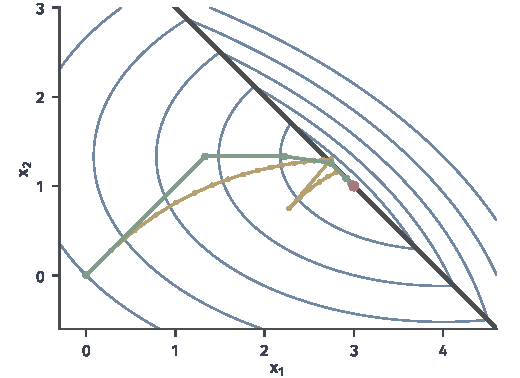
\includegraphics[width=88mm]{figures/05-optimization/06-constrained-optimization/matplotlib/pm-exact-ista/figure.pdf}
  \caption{二元例中一次罚$E_4$的两种解法，蓝线是等高线，深灰直线是约束。绿线是邻近梯度法（步长$1/3$），第三步落到直线上，此后沿直线走向红点。黄线是次梯度法（步长$0.07$），在直线两侧反复穿越，停留在解附近的一个小区域。}
  \label{fig:pm-exact-ista}
\end{BookInlineFigure}

\paragraph{一般约束的处理}
这个闭式解依赖约束只有一条且是线性的。若$\bm{h}(\bm{x})=\bm{A}\bm{x}-\bm{b}$有多行，$\lVert\bm{A}\bm{x}-\bm{b}\rVert_1$的邻近映射本身就要解一个优化问题；若$h_j$非线性，一般没有闭式解。

常用的办法是第~\ref{chap:nonsmooth-composite-optimization}章的局部模型：在当前点把约束线性化，保留绝对值，再加上二次距离项，解
\begin{equation}
 \min_{\bm{d}}\ \nabla f(\bm{x})^\top\bm{d}+\frac{1}{2\alpha}\lVert\bm{d}\rVert_2^2+\rho\sum_{j=1}^p\bigl\lvert h_j(\bm{x})+\nabla h_j(\bm{x})^\top\bm{d}\bigr\rvert .
 \label{eq:pm-exact-model}
\end{equation}
引入非负松弛变量把绝对值拆开，这是一个凸二次规划。模型是否可信要用真实的$E_\rho$检验，也就是比较预测下降和实际下降，第~\ref{chap:sequential-quadratic-programming}章会回到这一点。

解$E_\rho$结束时，还需要回到原问题做两项检查。第一，算出原约束的违规量$V(\bm{x})$，罚目标下降了不代表违规量已经降到容差以下。第二，核对$\rho$是否大于乘子估计的最大绝对分量。如果$\lvert\xi_j\rvert$贴着$1$，定理~\ref{thm:pm-exact-global}的条件就没有满足，应当增大$\rho$再解。数值上的$\rho$也不宜太大，否则目标的信息在罚项面前被淹没，迭代会贴着约束走得很慢。

\section{对偶上升}
\label{sec:pm-dual-ascent}

二次罚的解满足$\rho h(\bm{x}_\rho)\to\nu^\star$，一次罚的门槛也是乘子。两节下来，真正需要的量似乎一直是乘子，罚项只是在间接地把它制造出来。本节换一个问题：如果直接把乘子当作价格来调整，不加任何罚项，能走多远？

\paragraph{价格让碗倾斜}
先回到工厂的例子。总部报出乘子$\nu$，相当于对约束$x_1+x_2-4$计价，两家工厂面对的是Lagrange函数：
\[
 \mathcal{L}(\bm{x},\nu)=\frac12x_1^2+\frac32x_2^2+\nu(x_1+x_2-4).
\]
固定$\nu$，这是一个没有约束的严格凸二次函数。令梯度为零，得到
\begin{equation}
 \bm{x}(\nu)=-\nu\Bigl(1,\ \frac13\Bigr).
 \label{eq:pm-running-lagrange-min}
\end{equation}
写成$p=-\nu$更好读：单价$p$越高，工厂产量越高，$x_1=p$，$x_2=p/3$。线性项$\nu(x_1+x_2)$不改变碗的形状，只把碗底平移。

图~\ref{fig:pm-price-tilt}是平移的过程。$\nu=0$时碗底在原点，离约束很远。$\nu=-2.4$时碗底靠近直线，还差一点。$\nu=-3$时碗底恰好落在约束上的红点处，也就是原问题的解。这时不用任何约束，无约束最小点自己满足了约束。

\begin{BookInlineFigure}
  \centering
  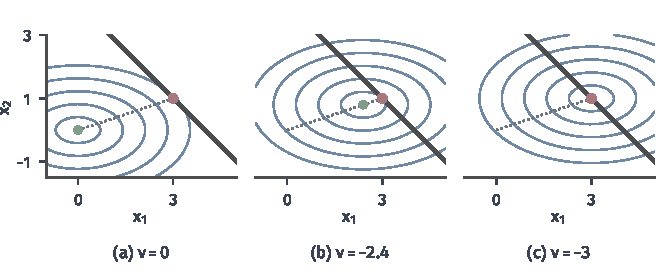
\includegraphics[width=112mm]{figures/05-optimization/06-constrained-optimization/matplotlib/pm-price-tilt/figure.pdf}
  \caption{乘子使Lagrange函数的碗底平移。蓝线是$\mathcal{L}(\cdot,\nu)$的等高线，深灰直线是约束，绿点是$\bm{x}(\nu)$，红点是解$(3,1)$，灰色点线是碗底走过的射线。(c)中$\nu=\nu^\star=-3$，碗底恰好落在约束上。}
  \label{fig:pm-price-tilt}
\end{BookInlineFigure}

把$\bm{x}(\nu)$代回，得到这个例子的对偶函数，它是Lagrange函数在$\bm{x}$上的最小值：
\[
 q(\nu)=\frac12\nu^2+\frac16\nu^2+\nu\Bigl(-\frac43\nu-4\Bigr).
\]
合并同类项，结果是
\begin{equation}
 q(\nu)=-\frac23\nu^2-4\nu .
 \label{eq:pm-running-dual}
\end{equation}
由弱对偶，每个$q(\nu)$都是$f^\star$的下界。这个二次函数在$\nu^\star=-3$处达到最大值$q(-3)=6=f^\star$。

\paragraph{一般情形}
一般问题中，固定$(\bm{\lambda},\bm{\nu})$，要解的是Lagrange子问题。第~\ref{chap:duality}章定义了对偶函数，这里允许把简单的集合$\bm{X}$（如整个空间或盒子）保留在子问题里：
\begin{equation}
 q(\bm{\lambda},\bm{\nu})=\inf_{\bm{x}\in\bm{X}}\mathcal{L}(\bm{x},\bm{\lambda},\bm{\nu}).
 \label{eq:pm-dual-function}
\end{equation}
它是一族关于$(\bm{\lambda},\bm{\nu})$的线性函数的下确界，因此总是凹的，这与原问题是否凸无关。求解对偶问题就是在$\bm{\lambda}\geq\bm{0}$上最大化这个凹函数。

\subsection{残差与乘子更新}
\label{sec:pm-dual-update}

要上升就要知道方向。这里的好消息是：解完Lagrange子问题，约束残差就是现成的上升信息。

\paragraph{残差是超梯度}
二元例的导数是$q'(\nu)=-\tfrac43\nu-4$，把式~\eqref{eq:pm-running-lagrange-min}代入，这恰好等于$h(\bm{x}(\nu))$。一般情形下$q$可能不可微，需要先推广“梯度”。

\begin{definition}[超梯度]
\label{def:pm-supergradient}
设$q$是凹函数，$\bm{y}$是定义域内一点。若向量$\bm{s}$使得对定义域内所有$\bm{y}'$都有
\begin{equation}
 q(\bm{y}')\leq q(\bm{y})+\langle\bm{s},\bm{y}'-\bm{y}\rangle,
 \label{eq:pm-supergradient}
\end{equation}
就称$\bm{s}$是$q$在$\bm{y}$处的\term{超梯度}（supergradient）。
\end{definition}

它就是$-q$的次梯度取负号：凹函数的图形总在这条切线下方。

\begin{theorem}[残差给出超梯度]
\label{thm:pm-residual-supergradient}
设$\bm{\lambda}\geq\bm{0}$，$\bar{\bm{x}}\in\bm{X}$是$\mathcal{L}(\cdot,\bm{\lambda},\bm{\nu})$在$\bm{X}$上的全局最小点。则$(\bm{g}(\bar{\bm{x}}),\bm{h}(\bar{\bm{x}}))$是$q$在$(\bm{\lambda},\bm{\nu})$处的一个超梯度。这里$\bm{g}=(g_1,\ldots,g_m)$，$\bm{h}=(h_1,\ldots,h_p)$，即对所有$\bm{\lambda}'$和$\bm{\nu}'$，有
\begin{equation}
 q(\bm{\lambda}',\bm{\nu}')\leq q(\bm{\lambda},\bm{\nu})+\langle\bm{g}(\bar{\bm{x}}),\bm{\lambda}'-\bm{\lambda}\rangle+\langle\bm{h}(\bar{\bm{x}}),\bm{\nu}'-\bm{\nu}\rangle .
 \label{eq:pm-residual-supergradient}
\end{equation}
\end{theorem}

\begin{proof}
$q$是下确界，所以它不超过任一点上的值：
\[
 q(\bm{\lambda}',\bm{\nu}')\leq\mathcal{L}(\bar{\bm{x}},\bm{\lambda}',\bm{\nu}').
\]
$\mathcal{L}$关于乘子是线性的，把乘子的差分拆出来：
\[
 \mathcal{L}(\bar{\bm{x}},\bm{\lambda}',\bm{\nu}')
 =\mathcal{L}(\bar{\bm{x}},\bm{\lambda},\bm{\nu})+\langle\bm{g}(\bar{\bm{x}}),\bm{\lambda}'-\bm{\lambda}\rangle+\langle\bm{h}(\bar{\bm{x}}),\bm{\nu}'-\bm{\nu}\rangle .
\]
$\bar{\bm{x}}$是全局最小点，所以上式右端第一项等于$q(\bm{\lambda},\bm{\nu})$。代入即得结论。
\end{proof}

证明中只有最后一步用到了最小点，而且必须是全局最小点。若$\bar{\bm{x}}$只是局部最小点，$\mathcal{L}(\bar{\bm{x}},\bm{\lambda},\bm{\nu})$比$q(\bm{\lambda},\bm{\nu})$大，式~\eqref{eq:pm-residual-supergradient}就失去了依据，残差不再是可靠的上升信息。若子问题只解到
\[
 \mathcal{L}(\bar{\bm{x}},\bm{\lambda},\bm{\nu})\leq q(\bm{\lambda},\bm{\nu})+\epsilon,
\]
同样的证明给出多一项$\epsilon$的不等式，$\mathcal{L}(\bar{\bm{x}},\bm{\lambda},\bm{\nu})-\epsilon$仍是可靠的下界。

\paragraph{主要思想}
沿超梯度走一步，不等式乘子投影回非负象限。这就是\term{对偶上升法}（dual ascent）：
\begin{equation}
 \begin{aligned}
 \bm{x}^{(t)}&\in\argmin_{\bm{x}\in\bm{X}}\mathcal{L}(\bm{x},\bm{\lambda}^{(t)},\bm{\nu}^{(t)}),\\
 \bm{\lambda}^{(t+1)}&=\bigl[\bm{\lambda}^{(t)}+\alpha^{(t)}\bm{g}(\bm{x}^{(t)})\bigr]_+,\\
 \bm{\nu}^{(t+1)}&=\bm{\nu}^{(t)}+\alpha^{(t)}\bm{h}(\bm{x}^{(t)}).
 \end{aligned}
 \label{eq:pm-dual-ascent}
\end{equation}
读法和定价一样。某条约束被违反，$g_i>0$，它的价格就上涨；有余量时，价格下降，但不能跌破零。等式约束的价格可正可负，没有截断。

\paragraph{计算过程}
用二元例走一遍，$\bm{X}=\mathbb{R}^2$。

\needspace{6\baselineskip}
\paragraph{变量}
\begin{itemize}
 \item $\bm{\nu}^{(t)}\in\mathbb{R}^p$：当前乘子。例中$p=1$。
 \item $\bm{x}^{(t)}\in\mathbb{R}^n$：Lagrange子问题的解。例中$n=2$。
 \item $\alpha^{(t)}>0$：乘子步长。
\end{itemize}

\paragraph{初始化}
取$\bm{\nu}^{(0)}$和步长。例中$\nu^{(0)}=0$，步长固定为$\alpha=0.6$，结束容差$\varepsilon=0.05$。

\needspace{6\baselineskip}
\paragraph{每轮更新}
\begin{enumerate}
 \item 解Lagrange子问题。例中用式~\eqref{eq:pm-running-lagrange-min}，第一轮
 \[
  \bm{x}^{(0)}=(0,0).
 \]
 \item 计算残差。例中第一轮
 \[
  h(\bm{x}^{(0)})=-4 .
 \]
 \item 按式~\eqref{eq:pm-dual-ascent}更新乘子。例中第一轮
 \[
  \nu^{(1)}=0+0.6\times(-4)=-2.4 .
 \]
\end{enumerate}
第二轮得到
\[
 \bm{x}^{(1)}=(2.4,\ 0.8),\qquad h(\bm{x}^{(1)})=-0.8,\qquad \nu^{(2)}=-2.88 .
\]
第三轮得到
\[
 \bm{x}^{(2)}=(2.88,\ 0.96),\qquad h(\bm{x}^{(2)})=-0.16,\qquad \nu^{(3)}=-2.976 .
\]
第四轮得到
\[
 \bm{x}^{(3)}=(2.976,\ 0.992),\qquad h(\bm{x}^{(3)})=-0.032 .
\]

结束条件是残差不超过$\varepsilon$，例中第四轮满足。最终得到的点是$\bm{x}^{(3)}=(2.976,\ 0.992)$，四轮对应的下界依次是
\[
 q(\nu^{(0)})=0,\quad q(\nu^{(1)})=5.76,\quad q(\nu^{(2)})=5.9904,\quad q(\nu^{(3)})\approx5.9996,
\]
单调升向$f^\star=6$。但是每一轮的$\bm{x}^{(t)}$都不可行。对偶上升改进的是下界，不是可行性。

\paragraph{步长的范围}
每轮更新代入后可以写成闭式。把$h(\bm{x}(\nu))=-\tfrac43\nu-4$代入，
\[
 \nu^{(t+1)}+3=\Bigl(1-\frac43\alpha\Bigr)(\nu^{(t)}+3).
\]
因此收敛当且仅当$\lvert1-\tfrac43\alpha\rvert<1$，也就是$0<\alpha<\tfrac32$。

图~\ref{fig:pm-dual-ascent}比较两个步长。$\alpha=0.6$时压缩因子是$0.2$，一步比一步接近顶点。$\alpha=1.5$恰好在边界上，因子是$-1$：乘子在$0$和$-6$之间永远跳动，$\bm{x}$在$(0,0)$和$(6,2)$之间跳动，两个点都不可行。

\begin{BookInlineFigure}
  \centering
  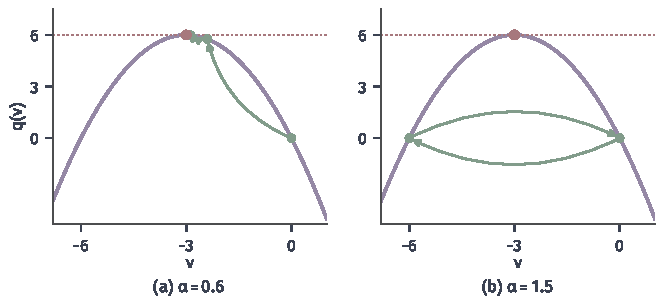
\includegraphics[width=112mm]{figures/05-optimization/06-constrained-optimization/matplotlib/pm-dual-ascent/figure.pdf}
  \caption{二元例中对偶函数$q(\nu)$（紫）上的对偶上升。绿点和箭头是乘子序列，从$\nu^{(0)}=0$出发，红点是最大点，红色点线是$f^\star=6$。(a)$\alpha=0.6$：压缩因子$0.2$，很快接近最大点。(b)$\alpha=1.5$：在$0$与$-6$之间反复跳动，不收敛。}
  \label{fig:pm-dual-ascent}
\end{BookInlineFigure}

\paragraph{可微的情形}
例子中的$q$是光滑的，这并非偶然。当$f$强凸、约束仿射时，子问题的解唯一，超梯度也唯一，对偶函数可以用第~\ref{chap:smooth-foundations}章的光滑分析。

\begin{theorem}[强凸目标的光滑对偶]
\label{thm:pm-smooth-dual}
设$f$连续可微且$\mu$强凸，$\bm{X}=\mathbb{R}^n$，约束为$\bm{A}\bm{x}=\bm{b}$。记$\bm{x}(\bm{\nu})$为$\mathcal{L}(\cdot,\bm{\nu})$的唯一最小点。则$q$可微，并且
\begin{equation}
 \nabla q(\bm{\nu})=\bm{A}\bm{x}(\bm{\nu})-\bm{b},
 \label{eq:pm-smooth-dual}
\end{equation}
其梯度满足
\begin{equation}
 \lVert\nabla q(\bm{\nu}_1)-\nabla q(\bm{\nu}_2)\rVert_2\leq\frac{\lVert\bm{A}\rVert_2^2}{\mu}\lVert\bm{\nu}_1-\bm{\nu}_2\rVert_2 .
 \label{eq:pm-smooth-dual-lipschitz}
\end{equation}
于是只要最优乘子存在，固定步长$0<\alpha<2\mu/\lVert\bm{A}\rVert_2^2$的对偶上升满足$q(\bm{\nu}^{(t)})\to d^\star$，其中$d^\star$是对偶最优值。
\end{theorem}

\begin{proof}
记$\bm{x}_k=\bm{x}(\bm{\nu}_k)$。驻定条件给出$\nabla f(\bm{x}_k)=-\bm{A}^\top\bm{\nu}_k$。由强凸性，
\[
 \mu\lVert\bm{x}_1-\bm{x}_2\rVert_2^2\leq\langle\nabla f(\bm{x}_1)-\nabla f(\bm{x}_2),\bm{x}_1-\bm{x}_2\rangle .
\]
把驻定条件代入，并用Cauchy--Schwarz不等式，得到
\[
 \mu\lVert\bm{x}_1-\bm{x}_2\rVert_2^2
 \leq-\langle\bm{\nu}_1-\bm{\nu}_2,\bm{A}(\bm{x}_1-\bm{x}_2)\rangle
 \leq\lVert\bm{A}\rVert_2\lVert\bm{\nu}_1-\bm{\nu}_2\rVert_2\lVert\bm{x}_1-\bm{x}_2\rVert_2 .
\]
两边约去一个因子，得到
\[
 \lVert\bm{x}_1-\bm{x}_2\rVert_2\leq\frac{\lVert\bm{A}\rVert_2}{\mu}\lVert\bm{\nu}_1-\bm{\nu}_2\rVert_2 .
\]

记$\bm{s}(\bm{\nu})=\bm{A}\bm{x}(\bm{\nu})-\bm{b}$。由上式，$\bm{s}$满足式~\eqref{eq:pm-smooth-dual-lipschitz}的Lipschitz界。

由定理~\ref{thm:pm-residual-supergradient}，$\bm{s}(\bm{\nu}_1)$和$\bm{s}(\bm{\nu}_2)$分别是两点的超梯度。对两点分别写一次超梯度不等式，得到
\[
 \langle\bm{s}(\bm{\nu}_2),\bm{\nu}_2-\bm{\nu}_1\rangle\leq q(\bm{\nu}_2)-q(\bm{\nu}_1)\leq\langle\bm{s}(\bm{\nu}_1),\bm{\nu}_2-\bm{\nu}_1\rangle .
\]
上下两端相差不超过$\lVert\bm{s}(\bm{\nu}_2)-\bm{s}(\bm{\nu}_1)\rVert_2\lVert\bm{\nu}_2-\bm{\nu}_1\rVert_2$，这是$\lVert\bm{\nu}_2-\bm{\nu}_1\rVert_2$的二阶量，所以$q$在$\bm{\nu}_1$处可微，梯度是$\bm{s}(\bm{\nu}_1)$。

最后，$-q$是光滑凸函数，步长范围内的梯度法收敛结论见第~\ref{chap:smooth-foundations}章和第~\ref{chap:first-order-methods}章。
\end{proof}

在二元例中，$\bm{A}=(1,1)$，$\lVert\bm{A}\rVert_2^2=2$，$f$的强凸常数$\mu=1$，定理的步长上限是$1$，比实际范围$\tfrac32$保守。这是因为定理把两个坐标方向的曲率都按最小值$\mu=1$估计，而实际的$\lvert q''\rvert$只有$\tfrac43$。

\paragraph{不可微的情形}
$f$不强凸时，子问题的解可能不唯一，$q$在这些点上有折角。下面的例子有两个变量和一条资源约束，后面还要继续使用：
\begin{equation}
 \min_{\bm{x}\in[0,1]^2}\ -x_1-x_2\qquad\text{s.t.}\qquad 2x_1+2x_2\leq3 .
 \label{eq:pm-lp-resource}
\end{equation}
它的最优值$f^\star=-1.5$，在$x_1+x_2=1.5$的线段上取得。固定$\lambda\geq0$，子问题对两个变量是分开的线性函数，每个变量的系数是$2\lambda-1$。

因此$\lambda<\tfrac12$时解是$(1,1)$，$\lambda>\tfrac12$时解是$(0,0)$，$\lambda=\tfrac12$时任意点都是解。代入得到对偶函数：
\[
 q(\lambda)=\begin{cases}\lambda-2,&\lambda\leq\tfrac12,\\-3\lambda,&\lambda\geq\tfrac12.\end{cases}
\]
$q$在$\lambda^\star=\tfrac12$处达到最大值$-1.5$，折角正好在最优点上。

超梯度步未必提高$q$。取$\alpha=0.12$，$\lambda^{(0)}=0$，乘子序列是
\[
 0,\ 0.12,\ 0.24,\ 0.36,\ 0.48,\ 0.60,\ 0.24,\ 0.36,\ 0.48,\ 0.60,\ldots
\]
对偶值$q(0.48)=-1.52$，下一步$q(0.60)=-1.8$，反而下降了。这与第~\ref{chap:nonsmooth-composite-optimization}章的次梯度法一样：步子越过折角就会下降，能保证的是到最优乘子的距离或者最好点的对偶值，而不是每步上升。图~\ref{fig:pm-primal-recovery}(a)中的绿点就在折角两侧来回。

\subsection{对偶分解与原始恢复}
\label{sec:pm-decomposition}

这一小节回答两个问题：对偶上升的计算好在哪里，以及算到最后怎样得到一个能用的原始解。

\paragraph{固定价格后各块分离}
设变量分成$K$块，目标按块可分，只有一条线性资源约束把它们联系起来：
\begin{equation}
 \min_{\bm{x}_k\in\bm{X}_k}\ \sum_{k=1}^Kf_k(\bm{x}_k)\qquad\text{s.t.}\qquad\sum_{k=1}^K\bm{A}_k\bm{x}_k\leq\bm{b}.
 \label{eq:pm-separable}
\end{equation}
固定乘子$\bm{\lambda}\geq\bm{0}$，Lagrange函数按块拆开：
\[
 \mathcal{L}(\bm{x},\bm{\lambda})=\sum_{k=1}^K\Bigl(f_k(\bm{x}_k)+\langle\bm{\lambda},\bm{A}_k\bm{x}_k\rangle\Bigr)-\langle\bm{\lambda},\bm{b}\rangle .
\]
和式中的每一项只含一块变量，所以$K$个子问题可以独立求解，互不通信。这种做法称为\term{对偶分解}（dual decomposition）。

协调者只做一件事：收集各块的用量$\bm{A}_k\bm{x}_k$，算出总残差，按下式更新价格：
\begin{equation}
 \bm{\lambda}^{(t+1)}=\Bigl[\bm{\lambda}^{(t)}+\alpha^{(t)}\Bigl(\sum_{k=1}^K\bm{A}_k\bm{x}_k^{(t)}-\bm{b}\Bigr)\Bigr]_+ .
 \label{eq:pm-decomposition-update}
\end{equation}
图~\ref{fig:pm-decomposition}以二元例为例，它本身就是两块问题：每家工厂只知道自己的成本和价格，协调者只知道总量和目标。

\begin{BookInlineFigure}
  \centering
  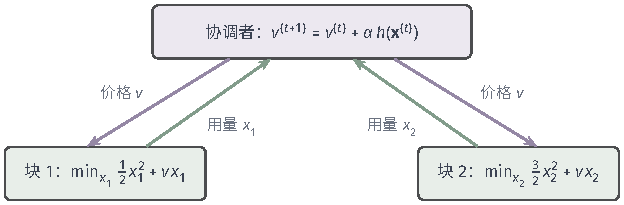
\includegraphics[width=105mm]{figures/05-optimization/06-constrained-optimization/tikz/pm-decomposition/figure.pdf}
  \caption{二元例的对偶分解。协调者（紫框）把当前价格$\nu$发给各块（紫色箭头），两块（绿框）独立求解自己的子问题，再把用量报回（绿色箭头）。协调者只用总量更新价格，不需要知道各块的成本函数。}
  \label{fig:pm-decomposition}
\end{BookInlineFigure}

分解改变的是计算的组织方式，算法在数学上仍是同一个对偶上升。收敛性质不因为分块而变好，第~\ref{chap:block-optimization}章处理的是目标本身不可分的分块，这里的分块靠乘子把约束解开。

\paragraph{原始点不可行}
继续看式~\eqref{eq:pm-lp-resource}。两个变量的子问题总是给出$(1,1)$或$(0,0)$。前者违反资源约束，$2x_1+2x_2=4>3$；后者可行，目标值却是$0$，离$f^\star$很远。图~\ref{fig:pm-primal-recovery}(b)的绿线就是这种情况：总量$x_1+x_2$一直在$2$和$0$之间跳，从不等于最优所需的$1.5$。

原因在于，对偶上升求的是价格，给定价格之后，解可以停在子问题解集的任何一点上。这个例子里，$\lambda^\star=\tfrac12$处的子问题有无穷多解，$q$的最大点却完全不告诉我们选哪个。

\paragraph{平均恢复}
第~\ref{chap:nonsmooth-composite-optimization}章在次梯度法上用过的平均，这里有直接的物理含义。把$\lambda$上涨的轮次看成资源用多了，下跌的轮次看成用少了，平均之后用量大致等于资源总量。图~\ref{fig:pm-primal-recovery}(b)的黄线是$x_1^{(t)}+x_2^{(t)}$的累积平均，它趋于$1.5$。

\begin{BookInlineFigure}
  \centering
  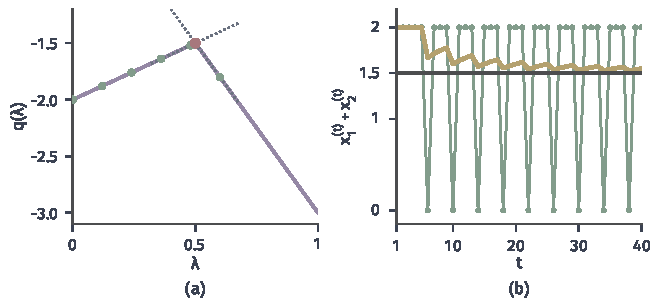
\includegraphics[width=112mm]{figures/05-optimization/06-constrained-optimization/matplotlib/pm-primal-recovery/figure.pdf}
  \caption{资源问题的超梯度上升，$\alpha=0.12$。(a)紫线是对偶函数，折角在$\lambda^\star=\tfrac12$，灰色点线是折角处的两条支撑线，绿点是前九个乘子，红点是最大点。(b)绿线是每轮的总量$x_1^{(t)}+x_2^{(t)}$，在$2$与$0$之间跳动；黄线是累积平均，深灰线是$1.5$。}
  \label{fig:pm-primal-recovery}
\end{BookInlineFigure}

\begin{theorem}[平均点的可行性与目标]
\label{thm:pm-primal-average}
设$f$和$g_i$在非空紧凸集$\bm{X}$上凸且连续，问题只有不等式约束，$f^\star$有限。设$\lVert\bm{g}(\bm{x})\rVert_2\leq S$对$\bm{x}\in\bm{X}$成立。从$\bm{\lambda}^{(0)}\geq\bm{0}$出发，取固定步长$\alpha>0$运行式~\eqref{eq:pm-dual-ascent}。记$\bar{\bm{x}}^{(T)}$为$\bm{x}^{(0)},\ldots,\bm{x}^{(T-1)}$的算术平均，则平均点在$\bm{X}$内，并且
\begin{equation}
 \bm{g}(\bar{\bm{x}}^{(T)})\leq\frac{\bm{\lambda}^{(T)}}{\alpha T},
 \label{eq:pm-average-feasibility}
\end{equation}
\begin{equation}
 f(\bar{\bm{x}}^{(T)})-f^\star\leq\frac{\lVert\bm{\lambda}^{(0)}\rVert_2^2}{2\alpha T}+\frac{\alpha S^2}{2}.
 \label{eq:pm-average-objective}
\end{equation}
\end{theorem}

\begin{proof}
先证可行性。投影只会让乘子变大，$[a]_+\geq a$，所以
\[
 \bm{\lambda}^{(t+1)}\geq\bm{\lambda}^{(t)}+\alpha\bm{g}(\bm{x}^{(t)}).
\]
对$t=0,\ldots,T-1$求和，得到
\[
 \alpha\sum_{t=0}^{T-1}\bm{g}(\bm{x}^{(t)})\leq\bm{\lambda}^{(T)}-\bm{\lambda}^{(0)}\leq\bm{\lambda}^{(T)}.
\]
每个$g_i$是凸函数，由Jensen不等式，平均点上的函数值不超过函数值的平均：
\[
 g_i(\bar{\bm{x}}^{(T)})\leq\frac1T\sum_{t=0}^{T-1}g_i(\bm{x}^{(t)}).
\]
两式结合，除以$\alpha T$，即得式~\eqref{eq:pm-average-feasibility}。

再证目标。投影到非负象限不增加与原点的距离，所以
\[
 \lVert\bm{\lambda}^{(t+1)}\rVert_2^2\leq\lVert\bm{\lambda}^{(t)}+\alpha\bm{g}(\bm{x}^{(t)})\rVert_2^2\leq\lVert\bm{\lambda}^{(t)}\rVert_2^2+2\alpha\langle\bm{\lambda}^{(t)},\bm{g}(\bm{x}^{(t)})\rangle+\alpha^2S^2 .
\]
由弱对偶和$\bm{x}^{(t)}$的定义，
\[
 f(\bm{x}^{(t)})+\langle\bm{\lambda}^{(t)},\bm{g}(\bm{x}^{(t)})\rangle=q(\bm{\lambda}^{(t)})\leq f^\star .
\]
从上式解出内积，代入前一个不等式，得到
\[
 f(\bm{x}^{(t)})-f^\star\leq\frac{\lVert\bm{\lambda}^{(t)}\rVert_2^2-\lVert\bm{\lambda}^{(t+1)}\rVert_2^2}{2\alpha}+\frac{\alpha S^2}{2}.
\]
对$t$求和，左边用Jensen不等式，右边裂项相消，去掉非正的$-\lVert\bm{\lambda}^{(T)}\rVert_2^2$，除以$T$即得式~\eqref{eq:pm-average-objective}。
\end{proof}

平均点的违规量由$\bm{\lambda}^{(T)}/(\alpha T)$控制，只要乘子序列有界，它就以$1/T$趋于零。Slater条件可以保证有界。设$\tilde{\bm{x}}\in\bm{X}$满足$g_i(\tilde{\bm{x}})\leq-\sigma<0$，并记$f_{\min}$为$f$在$\bm{X}$上的最小值。对偶函数不超过$\mathcal{L}$在$\tilde{\bm{x}}$处的值，由此得到
\[
 \langle\bm{\lambda}^{(t)},\bm{g}(\bm{x}^{(t)})\rangle=q(\bm{\lambda}^{(t)})-f(\bm{x}^{(t)})\leq f(\tilde{\bm{x}})-f_{\min}-\sigma\lVert\bm{\lambda}^{(t)}\rVert_1 .
\]
记
\[
 R=\frac{f(\tilde{\bm{x}})-f_{\min}+\alpha S^2/2}{\sigma}.
\]
代入证明中的距离递推可知，只要$\lVert\bm{\lambda}^{(t)}\rVert_1\geq R$，范数就不会增大；否则一步至多增加$\alpha S$。所以
\[
 \lVert\bm{\lambda}^{(t)}\rVert_2\leq\max\bigl\{\lVert\bm{\lambda}^{(0)}\rVert_2,\ R+\alpha S\bigr\}.
\]

式~\eqref{eq:pm-average-objective}只是单侧的界：$\bar{\bm{x}}^{(T)}$略微不可行时，目标值可能低于$f^\star$。

在问题~\eqref{eq:pm-lp-resource}中，乘子进入周期后每四轮有三轮是$(1,1)$，一轮是$(0,0)$，平均趋于$(\tfrac34,\tfrac34)$，$2x_1+2x_2$趋于$3$，恰好用尽资源。这组权重$\tfrac34,\tfrac14$是从对偶迭代的频率里读出来的，并没有事先知道。

\paragraph{非凸时的恢复与证书}
平均依赖可行集和目标的凸性。把式~\eqref{eq:pm-lp-resource}的变量改成$x_i\in\{0,1\}$，子问题和对偶函数都不变，最优乘子仍是$\tfrac12$，下界最多是$-1.5$。可平均点$(\tfrac34,\tfrac34)$不是整数点，平均在这里没有意义。

这时可以从访问过的点里挑选，或者另加一个简单的修复步骤，例如按边际价值贪心地放入物品，直到资源用尽。这里贪心得到$(1,0)$，目标值$-1$，可行。

此时的结论要如实报告：可行解给出上界$-1$，迭代中最好的对偶值给出下界$-1.52$，间隙不超过$0.52$。这个问题真实的最优值是$-1$，对偶下界不紧是非凸问题的常态，第~\ref{chap:duality}章称之为对偶间隙。任何情况下都应当同时报告原始可行性和这个间隙，单独一个收敛的对偶值不构成原问题的解。

\section{增广Lagrange法（ALM）}
\label{sec:pm-alm}

前面两条路各有缺陷。二次罚能增加法向曲率，把子问题变成好解的碗，但违规量要靠$\rho\to\infty$才能消失。对偶上升不增加任何曲率，步长稍大就振荡，目标线性时子问题甚至定不出解。把价格和罚款放在同一个函数里，能否在有限的$\rho$下得到解？

\paragraph{从力的平衡出发}
二次罚的驻点满足$\nabla f+\rho\bm{J}^\top\bm{h}=\bm{0}$。要平衡目标的力，$\rho\bm{h}$必须接近$\bm{\nu}^\star$，所以$\bm{h}$不能为零。如果事先在罚项里加上一个估计的力$\bm{\nu}$，那么只要$\bm{\nu}$足够接近$\bm{\nu}^\star$，弹簧几乎不用拉长。

工厂的语言是，总部既标出单价，又对偏离总量收罚款。单价负责提供大部分的调节力，罚款只负责修正单价还没估准的那一小部分。写成函数，就是在Lagrange函数上加残差平方。

\begin{definition}[增广Lagrange函数]
\label{def:pm-al}
对等式约束问题和$\rho>0$，\term{增广Lagrange函数}（augmented Lagrangian）是
\begin{equation}
 \mathcal{L}_\rho(\bm{x},\bm{\nu})=f(\bm{x})+\langle\bm{\nu},\bm{h}(\bm{x})\rangle+\frac{\rho}{2}\lVert\bm{h}(\bm{x})\rVert_2^2 .
 \label{eq:pm-al}
\end{equation}
\end{definition}

配方之后可以看出它的结构：
\begin{equation}
 \mathcal{L}_\rho(\bm{x},\bm{\nu})=f(\bm{x})+\frac{\rho}{2}\Bigl\lVert\bm{h}(\bm{x})+\frac{\bm{\nu}}{\rho}\Bigr\rVert_2^2-\frac{1}{2\rho}\lVert\bm{\nu}\rVert_2^2 .
 \label{eq:pm-al-square}
\end{equation}
最后一项与$\bm{x}$无关。所以固定$\bm{\nu}$时，增广Lagrange函数就是一个目标移位的二次罚：它不再要求$\bm{h}=\bm{0}$，而是把残差往$-\bm{\nu}/\rho$处拉。移位量选得对，平衡点上的残差就恰好是零。

\paragraph{同一个例子}
对二元例，固定$\nu$和$\rho$，增广Lagrange函数的驻定方程是
\[
 (1+\rho)x_1+\rho x_2=4\rho-\nu,\qquad \rho x_1+(3+\rho)x_2=4\rho-\nu .
\]
两式相减仍得$x_1=3x_2$。代回得到
\begin{equation}
 x_2=\frac{4\rho-\nu}{3+4\rho},\qquad x_1=3x_2 .
 \label{eq:pm-running-al-solution}
\end{equation}
残差因此是
\begin{equation}
 h(\bm{x})=4x_2-4=-\frac{4(\nu+3)}{3+4\rho}.
 \label{eq:pm-running-al-residual}
\end{equation}
和二次罚的式~\eqref{eq:pm-running-penalty-residual}比较，二次罚对应$\nu=0$，残差只能靠分母变大。这里分子含有因子$\nu-\nu^\star=\nu+3$：只要$\nu=-3$，无论$\rho$多小，残差都是零。

图~\ref{fig:pm-alm-center}固定$\rho=1.5$，只改变$\nu$。等高线的形状完全不变，因为Hessian不依赖$\nu$；变的是碗底的位置，$\nu=0$时离直线较远，$\nu=-2$时贴近直线，$\nu=-3$时恰好落在解上。对比图~\ref{fig:pm-penalty-contours}，那里要靠压扁碗才能靠近直线，这里碗的形状没有变。

\begin{BookInlineFigure}
  \centering
  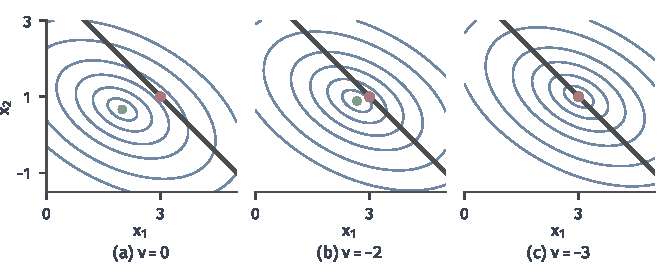
\includegraphics[width=112mm]{figures/05-optimization/06-constrained-optimization/matplotlib/pm-alm-center/figure.pdf}
  \caption{二元例中$\mathcal{L}_{1.5}(\cdot,\nu)$的等高线（蓝），$\rho=1.5$固定。深灰直线是约束，绿点是增广函数的最小点，红点是解$(3,1)$。改变乘子只平移碗底，不改变碗的形状；(c)$\nu=\nu^\star$时最小点落在解上。}
  \label{fig:pm-alm-center}
\end{BookInlineFigure}

这种现象不只在二次例子里出现，它在局部有一般的解释。下面的定理说，只要乘子是对的，有限的$\rho$就够了。

\begin{theorem}[最优乘子下的局部精确性]
\label{thm:pm-al-exact}
设$f,h_j$二阶连续可微，$(\bm{x}^\star,\bm{\nu}^\star)$满足KKT条件。记$\bm{W}$为$\mathcal{L}(\cdot,\bm{\nu}^\star)$在$\bm{x}^\star$处的Hessian，$\bm{J}=\bm{J}(\bm{x}^\star)$，并设对所有非零$\bm{d}$，只要$\bm{J}\bm{d}=\bm{0}$，就有$\bm{d}^\top\bm{W}\bm{d}>0$。则存在$\bar\rho\geq0$，使$\rho>\bar\rho$时，$\bm{x}^\star$是$\mathcal{L}_\rho(\cdot,\bm{\nu}^\star)$的严格局部最小点。
\end{theorem}

\begin{proof}
由$\bm{h}(\bm{x}^\star)=\bm{0}$和KKT条件，
\[
 \nabla_{\bm{x}}\mathcal{L}_\rho(\bm{x}^\star,\bm{\nu}^\star)=\nabla f+\bm{J}^\top\bm{\nu}^\star+\rho\bm{J}^\top\bm{h}=\bm{0}.
\]
含$h_j\nabla^2h_j$的项在$\bm{x}^\star$处为零，所以Hessian是
\[
 \nabla^2_{\bm{x}\bm{x}}\mathcal{L}_\rho(\bm{x}^\star,\bm{\nu}^\star)=\bm{W}+\rho\bm{J}^\top\bm{J}.
\]
只需证明$\rho$足够大时它正定。$\bm{J}^\top\bm{J}$半正定，这个矩阵关于$\rho$是单调的，一旦正定，更大的$\rho$也正定。

用反证法。若对每个正整数$k$，$\bm{W}+k\bm{J}^\top\bm{J}$都不正定，则存在单位向量$\bm{u}_k$，使
\[
 \bm{u}_k^\top\bm{W}\bm{u}_k+k\lVert\bm{J}\bm{u}_k\rVert_2^2\leq0 .
\]
单位向量的序列有收敛子列，设极限为$\bm{u}$。由上式得
\[
 \lVert\bm{J}\bm{u}_k\rVert_2^2\leq\frac{\lVert\bm{W}\rVert_2}{k}\to0 ,
\]
故$\bm{J}\bm{u}=\bm{0}$。

不等式的第二项非负，去掉它得$\bm{u}_k^\top\bm{W}\bm{u}_k\leq0$，取极限得$\bm{u}^\top\bm{W}\bm{u}\leq0$。这与假设矛盾，因为$\bm{u}\neq\bm{0}$且$\bm{J}\bm{u}=\bm{0}$。
\end{proof}

条件中$\bar\rho$的作用，看一个非凸的例子。取$f(\bm{x})=\tfrac12(x_1^2-x_2^2)$，$h(\bm{x})=x_2$，解是原点，$\nu^\star=0$。切方向是$x_1$轴，曲率$1>0$，满足二阶条件。此时增广函数的Hessian是$\operatorname{diag}(1,\rho-1)$，必须$\rho>1$才正定。$\rho<1$时，增广函数沿$x_2$方向没有下界。若$f$是凸函数且约束是线性的，就不需要这个门槛，任何$\rho>0$都行。

\subsection{原始变量与乘子更新}
\label{sec:pm-alm-update}

问题转到怎样得到正确的乘子。上一节的定理给了线索：用$\bm{\nu}$算出的增广函数的驻点，本身就告诉我们乘子该往哪里改。

\paragraph{主要思想}
对$\mathcal{L}_\rho$求梯度，把含$\bm{h}$的项合并，得到一个恒等式：
\begin{equation}
 \nabla_{\bm{x}}\mathcal{L}_\rho(\bm{x},\bm{\nu})=\nabla f(\bm{x})+\bm{J}(\bm{x})^\top\bigl(\bm{\nu}+\rho\bm{h}(\bm{x})\bigr)=\nabla_{\bm{x}}\mathcal{L}\bigl(\bm{x},\bm{\nu}+\rho\bm{h}(\bm{x})\bigr).
 \label{eq:pm-al-gradient-identity}
\end{equation}
如果$\bm{x}^{(t+1)}$是增广函数的驻点，那么它对应的Lagrange函数在乘子$\bm{\nu}^{(t)}+\rho\bm{h}(\bm{x}^{(t+1)})$处驻定。这个乘子把目标的力和约束的力平衡起来了，正好作为新的估计。

由此得到\term{增广Lagrange法}（augmented Lagrangian method，ALM）：
\begin{equation}
 \begin{aligned}
 \bm{x}^{(t+1)}&\approx\argmin_{\bm{x}}\mathcal{L}_{\rho}(\bm{x},\bm{\nu}^{(t)}),\\
 \bm{\nu}^{(t+1)}&=\bm{\nu}^{(t)}+\rho\,\bm{h}(\bm{x}^{(t+1)}).
 \end{aligned}
 \label{eq:pm-alm}
\end{equation}
这里$\rho$既是罚参数，也是乘子的步长。把步长取成$\rho$，正是恒等式~\eqref{eq:pm-al-gradient-identity}选出来的，不是任意的约定。

形式上它和对偶上升~\eqref{eq:pm-dual-ascent}只差一点：残差的取法。对偶上升先在旧乘子下解Lagrange子问题，用得到的残差算新乘子。ALM的$\bm{x}^{(t+1)}$满足的是新乘子下的驻定条件，残差实际上是在“走到之后的乘子”处读的。这正是第~\ref{chap:nonsmooth-composite-optimization}章显式步和隐式步的区别。

\begin{theorem}[ALM是对偶问题的邻近点法]
\label{thm:pm-alm-proximal}
设$f$是适当、闭的凸函数，$\bm{h}(\bm{x})=\bm{A}\bm{x}-\bm{b}$。设$\bm{x}^{+}$是$\mathcal{L}_\rho(\cdot,\bm{\nu})$的全局最小点，$\bm{\nu}^{+}=\bm{\nu}+\rho\bm{h}(\bm{x}^{+})$。则$\bm{x}^{+}$是$\mathcal{L}(\cdot,\bm{\nu}^{+})$的全局最小点，并且
\begin{equation}
 \bm{\nu}^{+}=\bm{\nu}+\rho\bm{s}^{+},\qquad \bm{s}^{+}=\bm{h}(\bm{x}^{+})\text{是}q\text{在}\bm{\nu}^{+}\text{处的超梯度},
 \label{eq:pm-alm-implicit}
\end{equation}
等价地，$\bm{\nu}^{+}$是下面问题的唯一解：
\begin{equation}
 \bm{\nu}^{+}=\argmax_{\bm{y}}\Bigl\{q(\bm{y})-\frac{1}{2\rho}\lVert\bm{y}-\bm{\nu}\rVert_2^2\Bigr\}.
 \label{eq:pm-alm-prox}
\end{equation}
\end{theorem}

\begin{proof}
$\bm{x}^{+}$最小化凸函数$\mathcal{L}_\rho(\cdot,\bm{\nu})$，最优性条件是
\[
 \bm{0}\in\partial f(\bm{x}^{+})+\bm{A}^\top\bigl(\bm{\nu}+\rho(\bm{A}\bm{x}^{+}-\bm{b})\bigr)=\partial f(\bm{x}^{+})+\bm{A}^\top\bm{\nu}^{+}.
\]
这正是凸函数$\mathcal{L}(\cdot,\bm{\nu}^{+})$在$\bm{x}^{+}$处的最优性条件，第一个结论成立。

由定理~\ref{thm:pm-residual-supergradient}，$\bm{s}^{+}=\bm{h}(\bm{x}^{+})$是$q$在$\bm{\nu}^{+}$处的超梯度，再由$\bm{\nu}^{+}$的定义得式~\eqref{eq:pm-alm-implicit}。

式~\eqref{eq:pm-alm-prox}中的目标强凹。它在$\bm{\nu}^{+}$处的最优性条件是$\bm{0}$属于$\partial q(\bm{\nu}^{+})-(\bm{\nu}^{+}-\bm{\nu})/\rho$，而式~\eqref{eq:pm-alm-implicit}正好给出这样一个超梯度。
\end{proof}

图~\ref{fig:pm-explicit-implicit}在二元例上比较两种步。$\rho=1.5$，从$\nu^{(0)}=0$出发，$q$的斜率是$-4$。显式步用当前点的斜率，走到$0+1.5\times(-4)=-6$，越过最大点，这就是图~\ref{fig:pm-dual-ascent}(b)的振荡。隐式步要求落点的斜率$s$满足$\nu^{+}=\nu+1.5s$，代入$s=-\tfrac43\nu^{+}-4$，解出$\nu^{+}=-2$，落在最大点的同一侧。

\begin{BookInlineFigure}
  \centering
  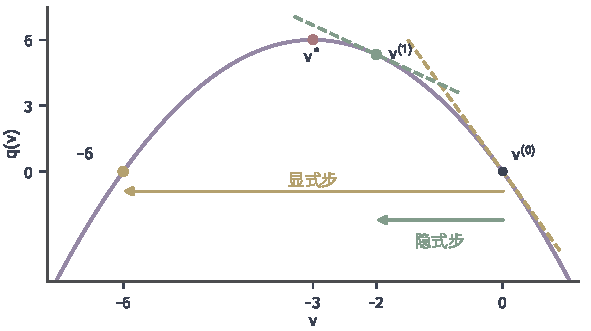
\includegraphics[width=100mm]{figures/05-optimization/06-constrained-optimization/matplotlib/pm-explicit-implicit/figure.pdf}
  \caption{同样的步长$\rho=1.5$下，对偶函数（紫）上的显式步与隐式步。黄色虚线是$\nu^{(0)}=0$处的切线，显式步按它的斜率走到$-6$（黄点）。绿色虚线是$\nu^{(1)}=-2$处的切线，隐式步要求落点切线的斜率与步长一致，得到绿点。红点是最大点$\nu^\star$。}
  \label{fig:pm-explicit-implicit}
\end{BookInlineFigure}

\begin{BookInlineTable}
  \centering
  \begin{tabular}{@{}lll@{}}
    \toprule
     & 对偶上升 & ALM\\
    \midrule
    原始子问题 & $\min\mathcal{L}(\cdot,\bm{\nu})$ & $\min\mathcal{L}_\rho(\cdot,\bm{\nu})$\\
    残差读取点 & 旧乘子（显式） & 新乘子（隐式）\\
    步长限制 & 受$q$的曲率限制 & 任意$\rho>0$（凸问题）\\
    子问题 & 目标可分则可分 & 平方项通常耦合各块\\
    目标线性时 & 子问题可能无解或解不唯一 & 平方项提供曲率\\
    \bottomrule
  \end{tabular}
  \caption{对偶上升与ALM的对照。ALM用更难的子问题换取稳定的乘子更新。}
  \label{tab:pm-dual-vs-alm}
\end{BookInlineTable}

压缩的速度可以显式写出。下面的定理针对最简单的等式约束二次规划，它的结论和图上的行为完全一致。

\begin{theorem}[线性等式二次问题的压缩率]
\label{thm:pm-alm-quadratic-rate}
设$f$是二次函数$\tfrac12\bm{x}^\top\bm{G}\bm{x}-\bm{d}^\top\bm{x}$，$\bm{G}\succ\bm{0}$，$\bm{h}(\bm{x})=\bm{A}\bm{x}-\bm{b}$，$\bm{A}$行满秩，记$\bm{S}=\bm{A}\bm{G}^{-1}\bm{A}^\top$。则精确求解子问题的ALM满足
\begin{equation}
 \bm{\nu}^{(t+1)}-\bm{\nu}^\star=(\bm{I}+\rho\bm{S})^{-1}(\bm{\nu}^{(t)}-\bm{\nu}^\star),
 \label{eq:pm-alm-linear-map}
\end{equation}
于是
\begin{equation}
 \lVert\bm{\nu}^{(t+1)}-\bm{\nu}^\star\rVert_2\leq\frac{1}{1+\rho\,\lambda_{\min}(\bm{S})}\lVert\bm{\nu}^{(t)}-\bm{\nu}^\star\rVert_2 .
 \label{eq:pm-alm-rate}
\end{equation}
\end{theorem}

\begin{proof}
由恒等式~\eqref{eq:pm-al-gradient-identity}，$\bm{x}^{(t+1)}$满足
\[
 \bm{G}\bm{x}^{(t+1)}-\bm{d}+\bm{A}^\top\bm{\nu}^{(t+1)}=\bm{0},
\]
解出
\[
 \bm{x}^{(t+1)}=\bm{G}^{-1}(\bm{d}-\bm{A}^\top\bm{\nu}^{(t+1)}).
\]
代入乘子更新式，得到
\[
 \bm{\nu}^{(t+1)}-\bm{\nu}^{(t)}=\rho\bigl(\bm{A}\bm{G}^{-1}\bm{d}-\bm{S}\bm{\nu}^{(t+1)}-\bm{b}\bigr).
\]
$\bm{\nu}^\star$满足同样形式的方程
\[
 \bm{A}\bm{G}^{-1}\bm{d}-\bm{S}\bm{\nu}^\star-\bm{b}=\bm{0},
\]
两式相减，得到
\[
 \bm{\nu}^{(t+1)}-\bm{\nu}^{(t)}=-\rho\bm{S}(\bm{\nu}^{(t+1)}-\bm{\nu}^\star).
\]
移项得
\[
 (\bm{I}+\rho\bm{S})(\bm{\nu}^{(t+1)}-\bm{\nu}^\star)=\bm{\nu}^{(t)}-\bm{\nu}^\star ,
\]
即式~\eqref{eq:pm-alm-linear-map}。$\bm{S}$对称正定，取范数即得式~\eqref{eq:pm-alm-rate}。
\end{proof}

二元例中$\bm{S}=1+\tfrac13=\tfrac43$，压缩因子是$3/(3+4\rho)$，$\rho=1.5$时为$\tfrac13$。任何$\rho>0$都是压缩的，和对偶上升要求$\alpha<\tfrac32$形成对比。

\paragraph{计算过程}
仍用二元例，并沿用第~\ref{sec:pm-rho-update}小节的外层容差。

\needspace{6\baselineskip}
\paragraph{变量}
\begin{itemize}
 \item $\bm{\nu}^{(t)}\in\mathbb{R}^p$：乘子估计。例中$p=1$。
 \item $\bm{x}^{(t)}\in\mathbb{R}^n$：增广子问题的解。例中$n=2$。
 \item $\rho>0$：罚参数，下一小节讨论它的调整。
\end{itemize}

\paragraph{初始化}
取$\bm{\nu}^{(0)}$和$\rho$。例中$\nu^{(0)}=0$，$\rho=1.5$，外层容差$\varepsilon=0.05$。

\needspace{6\baselineskip}
\paragraph{每轮更新}
\begin{enumerate}
 \item 近似最小化$\mathcal{L}_\rho(\cdot,\bm{\nu}^{(t)})$。例中由式~\eqref{eq:pm-running-al-solution}，$\rho=1.5$时$x_2=(6-\nu)/9$，第一轮
 \[
  \bm{x}^{(1)}=\Bigl(2,\ \frac23\Bigr).
 \]
 \item 计算残差。例中第一轮
 \[
  h(\bm{x}^{(1)})=-\frac43 .
 \]
 \item 由式~\eqref{eq:pm-alm}更新乘子。例中第一轮
 \[
  \nu^{(1)}=0+1.5\times\Bigl(-\frac43\Bigr)=-2 .
 \]
\end{enumerate}
第二轮得到
\[
 \bm{x}^{(2)}=\Bigl(\frac83,\ \frac89\Bigr),\qquad h(\bm{x}^{(2)})=-\frac49,\qquad \nu^{(2)}=-\frac83 .
\]
第三轮得到
\[
 \bm{x}^{(3)}=\Bigl(\frac{26}{9},\ \frac{26}{27}\Bigr),\qquad h(\bm{x}^{(3)})=-\frac{4}{27},\qquad \nu^{(3)}=-\frac{26}{9}.
\]
第四轮得到
\[
 \bm{x}^{(4)}=\Bigl(\frac{80}{27},\ \frac{80}{81}\Bigr),\qquad h(\bm{x}^{(4)})=-\frac{4}{81}\approx-0.049 .
\]

结束条件是$\lvert h\rvert\leq\varepsilon$，例中第四轮满足。最终得到$\bm{x}^{(4)}\approx(2.963,0.988)$，更新后的乘子是$\nu^{(4)}=-\tfrac{80}{27}\approx-2.963$。

第一轮和二次罚$\rho=1.5$的结果相同，因为此时$\nu=0$。此后二次罚换$\rho$，ALM换$\nu$。用相同的梯度法作内层，四轮分别用$21$、$18$、$15$、$12$步，共$66$步，$\rho$一直是$1.5$，条件数一直是$3.1$。

图~\ref{fig:pm-alm-vs-penalty}(a)比较两种方法。按外层轮数看，二次罚（$\rho$每轮乘$10$）下降得更快；但它每一轮都在解一个更病态的问题。ALM每轮只把残差缩小到$\tfrac13$，却始终在解同一个条件数很小的问题。(b)是ALM中$\rho$的取舍：$\rho$越大，外层压缩因子越小，轮数越少，内层条件数越大。

\begin{BookInlineFigure}
  \centering
  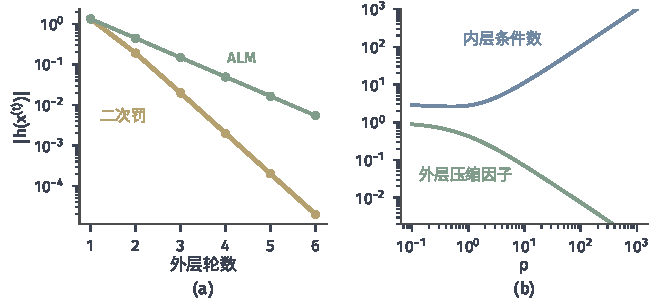
\includegraphics[width=112mm]{figures/05-optimization/06-constrained-optimization/matplotlib/pm-alm-vs-penalty/figure.pdf}
  \caption{二元例上ALM与二次罚的对比。(a)半对数坐标下的约束残差：黄线是二次罚（$\rho$从$1.5$开始每轮乘$10$），绿线是ALM（$\rho=1.5$固定），每轮精确求解。(b)双对数坐标，绿线是ALM的外层压缩因子$3/(3+4\rho)$，蓝线是内层Hessian的条件数。}
  \label{fig:pm-alm-vs-penalty}
\end{BookInlineFigure}

\paragraph{不等式约束}
前面的公式都是等式约束，不等式约束的乘子有符号限制，不能直接照搬。标准的做法是加入非负松弛变量，把$g_i(\bm{x})\leq0$写成$g_i(\bm{x})+s_i=0$，$s_i\geq0$，然后只对这个等式写增广函数。

固定$\bm{x}$，把$s_i$的优化解出来。对第$i$条约束，要在$s_i\geq0$上最小化
\[
 \lambda_i(g_i+s_i)+\frac\rho2(g_i+s_i)^2 .
\]
这是$s_i$的凸二次函数，无约束极小点是$-g_i-\lambda_i/\rho$，投影到非负数后得到
\[
 s_i=\Bigl[-g_i-\frac{\lambda_i}{\rho}\Bigr]_+ .
\]
由此可得$g_i+s_i=\max\{g_i,-\lambda_i/\rho\}$。把它代回去，分$g_i\geq-\lambda_i/\rho$和$g_i<-\lambda_i/\rho$两种情形合并，增广函数为
\begin{equation}
 \mathcal{L}_\rho(\bm{x},\bm{\lambda})=f(\bm{x})+\frac{1}{2\rho}\sum_{i=1}^m\Bigl([\lambda_i+\rho g_i(\bm{x})]_+^2-\lambda_i^2\Bigr).
 \label{eq:pm-al-inequality}
\end{equation}
乘子沿松弛等式更新，$\lambda_i^{+}=\lambda_i+\rho(g_i+s_i)$，整理后是
\begin{equation}
 \lambda_i^{+}=\bigl[\lambda_i+\rho g_i(\bm{x})\bigr]_+ .
 \label{eq:pm-alm-inequality-update}
\end{equation}

这个公式自动带来了对偶可行和互补。$\lambda_i^{+}$是正部，所以非负。若$g_i<-\lambda_i/\rho$，约束有足够余量，$\lambda_i^{+}=0$，该约束暂时不起作用。不动点$\lambda_i^{+}=\lambda_i$等价于$\max\{g_i,-\lambda_i/\rho\}=0$，它恰好是
\begin{equation}
 g_i\leq0,\qquad \lambda_i\geq0,\qquad \lambda_ig_i=0 .
 \label{eq:pm-complementarity}
\end{equation}
图~\ref{fig:pm-alm-ineq}(a)是单条约束的代价：在$g\geq-\lambda/\rho$一侧是二次增长的曲线，另一侧是常数$-\lambda^2/(2\rho)$，两段光滑相接。(b)是乘子更新，折线在$-\lambda/\rho$处把负值截断。

\begin{BookInlineFigure}
  \centering
  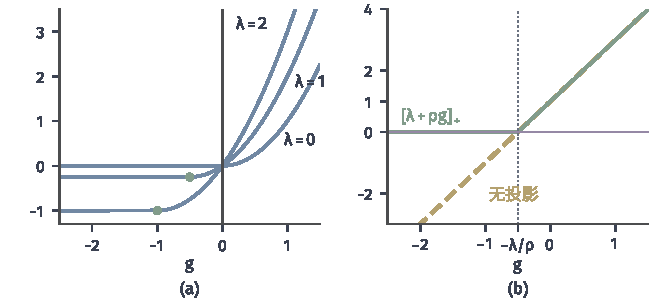
\includegraphics[width=112mm]{figures/05-optimization/06-constrained-optimization/matplotlib/pm-alm-ineq/figure.pdf}
  \caption{不等式约束的增广项，$\rho=2$。(a)蓝线是$([\lambda+\rho g]_+^2-\lambda^2)/(2\rho)$关于$g$的曲线，$\lambda=0,1,2$，绿点是分段点$g=-\lambda/\rho$，深灰竖线是约束边界。(b)$\lambda=1$的乘子更新：绿线是投影形式$[\lambda+\rho g]_+$，黄色虚线是不作投影的直线，紫线是零。}
  \label{fig:pm-alm-ineq}
\end{BookInlineFigure}

用一维例检验。式~\eqref{eq:pm-one-dim}的$g=1-x$，式~\eqref{eq:pm-al-inequality}对$x$的导数是
\[
 1-[\lambda+\rho(1-x)]_+ .
\]
令其为零，得到
\[
 x=1+\frac{\lambda-1}{\rho}.
\]
此时$\lambda+\rho(1-x)=1$，所以由式~\eqref{eq:pm-alm-inequality-update}，不管$\lambda$从哪里开始，一次更新后都有$\lambda^{+}=1=\lambda^\star$。第二轮代入，$x=1$，就是原问题的解。二次罚在同一例上永远差$1/\rho$。

不作投影会出错。考虑$\min x^2$，$x\geq-1$，解$x^\star=0$，约束不活动，$\lambda^\star=0$。写$g=-1-x$，取$\rho=2$，$\lambda^{(0)}=0$。式~\eqref{eq:pm-alm-inequality-update}给出$\lambda^{+}=0$，一步就对。

若把它当作等式，用不带投影的公式，子问题的解是$x=(\lambda-2)/4$，乘子递推是$\lambda^{+}=\tfrac12\lambda-1$。序列$\lambda=0,-1,-1.5,\ldots$趋于$-2$，$x$趋于$-1$。这是把约束当作$x=-1$时的解，既不是原问题的解，乘子的符号也错了。

\subsection{参数与停止条件}
\label{sec:pm-alm-parameters}

ALM的结构已经确定，剩下三件事：什么时候放大$\rho$，子问题解到多准，什么时候算结束。

\paragraph{罚参数}
不必让$\rho$趋于无穷，但也不能太小。$\rho$太小时，一方面非凸问题的子问题可能无下界，另一方面外层压缩很慢。常用的规则是观察约束残差是否下降到位。把等式残差和不等式残差放在同一个向量里：
\begin{equation}
 \bm{c}^{(t)}=\Bigl(\bm{h}(\bm{x}^{(t)}),\ \max\bigl\{\bm{g}(\bm{x}^{(t)}),-\bm{\lambda}^{(t-1)}/\rho^{(t-1)}\bigr\}\Bigr),
 \label{eq:pm-alm-residual-vector}
\end{equation}
其中$\max$按分量取。它把不活动约束的残差也按互补要求记为零。若
\begin{equation}
 \lVert\bm{c}^{(t+1)}\rVert_2>\theta\lVert\bm{c}^{(t)}\rVert_2,
 \label{eq:pm-alm-rho-test}
\end{equation}
说明残差下降不够，令$\rho\leftarrow\beta\rho$，否则保持$\rho$不变。常见取值是$\theta\in[0.25,0.5]$，$\beta\in[2,10]$。

顺序上，先用当前的$\rho$更新乘子，再放大$\rho$。乘子本身是一个不依赖$\rho$的量，放大$\rho$不需要换算它。

例如二元例若从$\rho=0.15$开始，压缩因子是$3/3.6\approx0.83$。第一轮和第二轮的结果为
\[
 h(\bm{x}^{(1)})=-\frac{10}{3},\qquad h(\bm{x}^{(2)})=-\frac{25}{9}.
\]
第二轮的残差比是$0.83$，大于$\theta=0.5$，所以把$\rho$放大到$1.5$，此后压缩因子变成$\tfrac13$。

\paragraph{内层精度}
恒等式~\eqref{eq:pm-al-gradient-identity}给出了一个便利之处：增广函数的内层梯度$\lVert\nabla_{\bm{x}}\mathcal{L}_\rho(\bm{x},\bm{\nu}^{(t)})\rVert_2$，正是更新后的乘子下Lagrange驻定残差。所以内层容差就是外层驻定精度，不用另算。

外层初期乘子还不准，把子问题解得太细是浪费。常用的安排是让内层容差$\omega^{(t)}$随外层逐步收紧，最终降到所需的驻定精度。对凸问题，邻近点法的分析要求内层误差可和，$\sum_t\epsilon^{(t)}<\infty$；实现上也常用与约束残差挂钩的相对准则。

\paragraph{三类残差}
结束时要分别检查三项，任何一项不合格都不算解好：
\begin{equation}
 \begin{aligned}
 \text{原始可行：}\quad&\lVert\bm{h}(\bm{x})\rVert_2,\ \ \lVert[\bm{g}(\bm{x})]_+\rVert_2\leq\varepsilon_{\mathrm{p}},\\
 \text{Lagrange驻定：}\quad&\lVert\nabla_{\bm{x}}\mathcal{L}(\bm{x},\bm{\lambda}^{+},\bm{\nu}^{+})\rVert_2\leq\varepsilon_{\mathrm{d}},\\
 \text{互补：}\quad&\lVert\min\{-\bm{g}(\bm{x}),\bm{\lambda}^{+}\}\rVert_2\leq\varepsilon_{\mathrm{c}}.
 \end{aligned}
 \label{eq:pm-alm-stopping}
\end{equation}
其中$\min$按分量取，它为零当且仅当式~\eqref{eq:pm-complementarity}成立。式中的第二项对应恒等式~\eqref{eq:pm-al-gradient-identity}，第一项不会因为内层解得准而自动变小，这一点和二次罚相同。

\paragraph{能保证什么}
ALM的保证分成三个层次，所需条件依次不同。先证明凸问题的情形，证明本身也说明了$\rho$为什么影响外层。

\begin{theorem}[凸问题的固定参数收敛]
\label{thm:pm-alm-convex}
设$f$是适当、闭的凸函数，$\bm{h}(\bm{x})=\bm{A}\bm{x}-\bm{b}$，存在最优解和最优乘子$\bm{\nu}^\star$，且强对偶成立。设$\rho>0$固定，各子问题的全局最小点存在且精确求解，$\bm{s}^{(t)}=\bm{h}(\bm{x}^{(t)})$。则
\begin{equation}
 \sum_{t\geq1}\rho^2\lVert\bm{s}^{(t)}\rVert_2^2\leq\lVert\bm{\nu}^{(0)}-\bm{\nu}^\star\rVert_2^2,
 \label{eq:pm-alm-summable}
\end{equation}
并且$\bm{h}(\bm{x}^{(t)})\to\bm{0}$，$q(\bm{\nu}^{(t)})\to d^\star$，$f(\bm{x}^{(t)})\to f^\star$。
\end{theorem}

\begin{proof}
记$\bm{\nu}=\bm{\nu}^{(t-1)}$，$\bm{\nu}^{+}=\bm{\nu}^{(t)}$，$\bm{s}^{+}=\bm{s}^{(t)}$。由定理~\ref{thm:pm-alm-proximal}，$\bm{s}^{+}$是$q$在$\bm{\nu}^{+}$处的超梯度。在式~\eqref{eq:pm-supergradient}中取比较点$\bm{\nu}^\star$，得到
\[
 q(\bm{\nu}^\star)\leq q(\bm{\nu}^{+})+\langle\bm{s}^{+},\bm{\nu}^\star-\bm{\nu}^{+}\rangle .
\]
$\bm{\nu}^\star$是$q$的最大点，所以$q(\bm{\nu}^{+})\leq q(\bm{\nu}^\star)$，上式给出
\[
 \langle\bm{s}^{+},\bm{\nu}^{+}-\bm{\nu}^\star\rangle\leq0 .
\]
现在把$\bm{\nu}=\bm{\nu}^{+}-\rho\bm{s}^{+}$代入$\lVert\bm{\nu}-\bm{\nu}^\star\rVert_2^2$并展开：
\[
 \lVert\bm{\nu}-\bm{\nu}^\star\rVert_2^2=\lVert\bm{\nu}^{+}-\bm{\nu}^\star\rVert_2^2-2\rho\langle\bm{s}^{+},\bm{\nu}^{+}-\bm{\nu}^\star\rangle+\rho^2\lVert\bm{s}^{+}\rVert_2^2 .
\]
中间项非负，舍去后得到
\[
 \lVert\bm{\nu}^{+}-\bm{\nu}^\star\rVert_2^2+\rho^2\lVert\bm{s}^{+}\rVert_2^2\leq\lVert\bm{\nu}-\bm{\nu}^\star\rVert_2^2 .
\]
对$t$求和裂项，即得式~\eqref{eq:pm-alm-summable}，于是$\bm{s}^{(t)}\to\bm{0}$，且$\bm{\nu}^{(t)}$有界。

再由第一个不等式，
\[
 0\leq d^\star-q(\bm{\nu}^{+})\leq\langle\bm{s}^{+},\bm{\nu}^\star-\bm{\nu}^{+}\rangle\leq\lVert\bm{s}^{+}\rVert_2\lVert\bm{\nu}^\star-\bm{\nu}^{+}\rVert_2\to0 .
\]
最后，由定理~\ref{thm:pm-alm-proximal}，$\bm{x}^{(t)}$是$\mathcal{L}(\cdot,\bm{\nu}^{(t)})$的全局最小点，所以
\[
 f(\bm{x}^{(t)})=q(\bm{\nu}^{(t)})-\langle\bm{\nu}^{(t)},\bm{s}^{(t)}\rangle ,
\]
右边趋于$d^\star=f^\star$。
\end{proof}

式~\eqref{eq:pm-alm-summable}中的$\rho^2$说明，$\rho$越大，残差平方的总和越小，外层越快。定理既不要求$\rho$放大，也不要求$f$可微，并且$\bm{x}^{(t)}$本身不一定收敛，$f$不强凸时子问题的解可以不唯一。

非凸问题只有局部结论。设$(\bm{x}^\star,\bm{\nu}^\star)$满足KKT条件，LICQ和二阶充分条件成立。那么存在$\bar\rho$，当$\rho\geq\bar\rho$时，从足够接近$\bm{\nu}^\star$的乘子出发，取$\mathcal{L}_\rho$在$\bm{x}^\star$附近的局部最小点，乘子序列线性收敛到$\bm{\nu}^\star$，压缩因子约为$O(1/\rho)$。这一结论的证明需要对驻定方程应用隐函数定理，篇幅较长，读者可查阅Nocedal和Wright的著作\scite{math-nocedal2006numerical}，它的机制和式~\eqref{eq:pm-alm-rate}相同。

全局层次的结果最弱。若每个子问题只解到近似驻点，乘子保持有界（常把估计截断在一个大盒子里），可以证明聚点要么是约束违规量的驻点，要么在相应约束资格下是KKT点；和定理~\ref{thm:pm-quadratic-approximate}的结论是同一类型。只有每个子问题都取全局最小点，才能得到全局最优的结论，非凸问题通常做不到。下表把三个层次放在一起。

\begin{BookInlineTable}
  \centering
  \small
  \begin{tabular}{@{}lll@{}}
    \toprule
    情形 & 主要条件 & 结论\\
    \midrule
    凸，固定$\rho$ & 强对偶，子问题精确 & 残差趋零，目标值收敛\\
    非凸，局部 & LICQ，二阶充分，$\rho\geq\bar\rho$ & 乘子局部线性收敛\\
    非凸，全局策略 & 近似驻点，乘子有界 & 聚点为不可行驻点或KKT点\\
    \bottomrule
  \end{tabular}
  \caption{ALM的三层保证。下面一行不能推出上面两行的结论。}
  \label{tab:pm-alm-guarantees}
\end{BookInlineTable}

\section{交替方向乘子法（ADMM）}
\label{sec:pm-admm}

ALM的子问题比对偶上升的子问题难的地方，在于平方项把各块耦合了。于是要问：当目标由两块组成，能否既保留乘子带来的稳定性，又把两块分开计算？本节的问题形式是
\begin{equation}
 \min_{\bm{x},\bm{z}}\ f(\bm{x})+g(\bm{z})\qquad\text{s.t.}\qquad\bm{A}\bm{x}+\bm{B}\bm{z}=\bm{c},
 \label{eq:pm-admm-problem}
\end{equation}
其中$\bm{x}\in\mathbb{R}^n$，$\bm{z}\in\mathbb{R}^l$，$\bm{A}\in\mathbb{R}^{p\times n}$，$\bm{B}\in\mathbb{R}^{p\times l}$，$\bm{c}\in\mathbb{R}^p$。这里的$g$是第二块目标，不是不等式约束。对应的增广Lagrange函数是
\begin{equation}
 \mathcal{L}_\rho(\bm{x},\bm{z},\bm{\nu})=f(\bm{x})+g(\bm{z})+\langle\bm{\nu},\bm{A}\bm{x}+\bm{B}\bm{z}-\bm{c}\rangle+\frac\rho2\lVert\bm{A}\bm{x}+\bm{B}\bm{z}-\bm{c}\rVert_2^2 .
 \label{eq:pm-admm-al}
\end{equation}

\paragraph{平方项破坏了可分性}
对偶分解能并行，靠的是Lagrange函数按块可分。增广函数的平方项里有交叉项$\rho\langle\bm{A}\bm{x},\bm{B}\bm{z}\rangle$，可分性被破坏。ALM只能把$(\bm{x},\bm{z})$联合起来最小化，即使$f$和$g$各自都很简单。

\term{交替方向乘子法}（alternating direction method of multipliers，ADMM）的想法是：不把子问题解到最优，只把$\bm{x}$和$\bm{z}$各自更新一次，然后立即更新乘子。

这个想法要付代价。用二元例说明，把它看成$f(x)=\tfrac12x^2$，$g(z)=\tfrac32z^2$，$x+z=4$，$\rho=1.5$，$\nu=0$。联合最小化$\mathcal{L}_\rho$得到式~\eqref{eq:pm-running-al-solution}，即$(x,z)=(2,\tfrac23)$。

从$(0,0)$开始交替一次：先固定$z=0$，对$x$最小化，$x=\tfrac{\rho\cdot4}{1+\rho}=2.4$；再固定$x=2.4$，对$z$最小化，$z=\tfrac{\rho(4-2.4)}{3+\rho}=\tfrac{8}{15}$。结果是$(2.4,\tfrac{8}{15})$，与联合解$(2,\tfrac23)$不同。

图~\ref{fig:pm-admm-sweep}(a)画出了这两步：黄色折线先水平走，再竖直走，两步都只顾自己的方向，没有到达碗底。一次交替扫过两块，不等于把子问题解到最优，所以不能把ALM的结论直接搬过来。(b)是多轮的路径，ADMM走的是折线，ALM走的是直线，两者最后都到达红点。

\begin{BookInlineFigure}
  \centering
  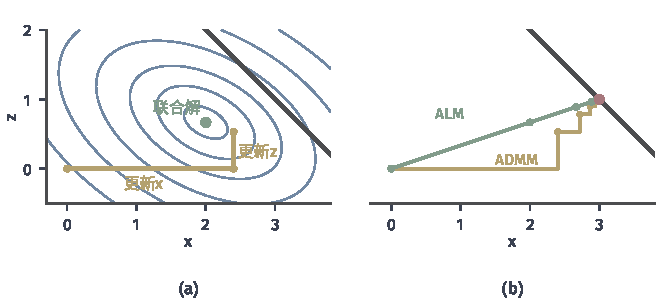
\includegraphics[width=112mm]{figures/05-optimization/06-constrained-optimization/matplotlib/pm-admm-sweep/figure.pdf}
  \caption{二元例上ADMM的两块交替更新，$\rho=1.5$。深灰直线是约束。(a)蓝线是$\nu=0$时增广函数的等高线，绿点是联合最小点$(2,\tfrac23)$，黄色折线是从原点出发的一次交替，停在$(2.4,\tfrac{8}{15})$。(b)绿线是ALM每轮的联合解，黄线是ADMM的折线路径，红点是解$(3,1)$。}
  \label{fig:pm-admm-sweep}
\end{BookInlineFigure}

\subsection{两块交替更新}
\label{sec:pm-admm-update}

\paragraph{主要思想}
每轮按固定的顺序做三步，后一步使用前一步刚得到的结果，如图~\ref{fig:pm-admm-flow}所示：
\begin{equation}
 \begin{aligned}
 \bm{x}^{(t+1)}&\in\argmin_{\bm{x}}\mathcal{L}_\rho(\bm{x},\bm{z}^{(t)},\bm{\nu}^{(t)}),\\
 \bm{z}^{(t+1)}&\in\argmin_{\bm{z}}\mathcal{L}_\rho(\bm{x}^{(t+1)},\bm{z},\bm{\nu}^{(t)}),\\
 \bm{\nu}^{(t+1)}&=\bm{\nu}^{(t)}+\rho\bigl(\bm{A}\bm{x}^{(t+1)}+\bm{B}\bm{z}^{(t+1)}-\bm{c}\bigr).
 \end{aligned}
 \label{eq:pm-admm}
\end{equation}

\begin{BookInlineFigure}
  \centering
  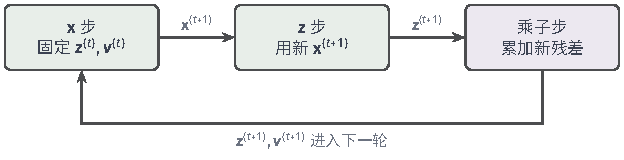
\includegraphics[width=105mm]{figures/05-optimization/06-constrained-optimization/tikz/pm-admm-flow/figure.pdf}
  \caption{ADMM一轮的三步。绿框是两个原始变量的最小化，后一块使用前一块的新值；紫框按新残差累加乘子。与ALM的区别在于$\bm{x}$和$\bm{z}$不联合求解。}
  \label{fig:pm-admm-flow}
\end{BookInlineFigure}

这和第~\ref{chap:block-optimization}章的分块最小化很像：在固定的目标上逐块求最小。两者的区别在于这里有线性耦合约束，单纯的分块下降可能卡在不是解的点上，ADMM靠乘子一步把约束信息累加进下一轮。

\paragraph{缩放乘子}
把乘子除以$\rho$，公式会简短很多。记残差$\bm{r}=\bm{A}\bm{x}+\bm{B}\bm{z}-\bm{c}$，配方得
\[
 \langle\bm{\nu},\bm{r}\rangle+\frac\rho2\lVert\bm{r}\rVert_2^2=\frac\rho2\lVert\bm{r}+\bm{u}\rVert_2^2-\frac\rho2\lVert\bm{u}\rVert_2^2,\qquad\bm{u}=\frac{\bm{\nu}}{\rho}.
\]

$\bm{u}$称为\term{缩放乘子}（scaled dual variable）。式~\eqref{eq:pm-admm}写成缩放形式是
\begin{equation}
 \begin{aligned}
 \bm{x}^{(t+1)}&\in\argmin_{\bm{x}}\ f(\bm{x})+\frac\rho2\lVert\bm{A}\bm{x}+\bm{B}\bm{z}^{(t)}-\bm{c}+\bm{u}^{(t)}\rVert_2^2,\\
 \bm{z}^{(t+1)}&\in\argmin_{\bm{z}}\ g(\bm{z})+\frac\rho2\lVert\bm{A}\bm{x}^{(t+1)}+\bm{B}\bm{z}-\bm{c}+\bm{u}^{(t)}\rVert_2^2,\\
 \bm{u}^{(t+1)}&=\bm{u}^{(t)}+\bm{A}\bm{x}^{(t+1)}+\bm{B}\bm{z}^{(t+1)}-\bm{c}.
 \end{aligned}
 \label{eq:pm-admm-scaled}
\end{equation}
两种写法完全等价。缩放乘子就是残差的累加和，这是它最直观的含义：$\bm{u}^{(t)}$记录到目前为止累计的残差。

\paragraph{套索问题的拆分}
ADMM的用处是把一个有结构的问题拆成两个容易的问题。第~\ref{chap:nonsmooth-composite-optimization}章的套索问题是
\begin{equation}
 \min_{\bm{x}}\ \frac12\lVert\bm{D}\bm{x}-\bm{y}\rVert_2^2+\gamma\lVert\bm{x}\rVert_1 ,
 \label{eq:pm-lasso}
\end{equation}
其中$\bm{D}\in\mathbb{R}^{N\times n}$，$\gamma>0$。把变量复制一份，让$f$负责最小二乘项$\tfrac12\lVert\bm{D}\bm{x}-\bm{y}\rVert_2^2$，$g$负责$\gamma\lVert\bm{z}\rVert_1$，并加上约束$\bm{x}-\bm{z}=\bm{0}$。这对应$\bm{A}=\bm{I}$，$\bm{B}=-\bm{I}$，$\bm{c}=\bm{0}$。

把$f$代入式~\eqref{eq:pm-admm-scaled}的第一行，这是一个二次子问题，解为
\begin{equation}
 \bm{x}^{(t+1)}=(\bm{D}^\top\bm{D}+\rho\bm{I})^{-1}\bigl(\bm{D}^\top\bm{y}+\rho(\bm{z}^{(t)}-\bm{u}^{(t)})\bigr).
 \label{eq:pm-lasso-x}
\end{equation}
第二行是$\gamma\lVert\bm{z}\rVert_1$加上一个以$\bm{x}^{(t+1)}+\bm{u}^{(t)}$为中心的二次项，按坐标可分，由软阈值给出：
\begin{equation}
 \bm{z}^{(t+1)}=S_{\gamma/\rho}\bigl(\bm{x}^{(t+1)}+\bm{u}^{(t)}\bigr),\qquad
 S_\tau(a)=\operatorname{sign}(a)\max\{\lvert a\rvert-\tau,0\}.
 \label{eq:pm-lasso-z}
\end{equation}
第三行是缩放乘子的累加：
\begin{equation}
 \bm{u}^{(t+1)}=\bm{u}^{(t)}+\bm{x}^{(t+1)}-\bm{z}^{(t+1)}.
 \label{eq:pm-lasso-u}
\end{equation}
二次子问题只含$f$，软阈值只含$g$，这样两部分结构都得到了利用。

\paragraph{计算过程}
用第~\ref{chap:nonsmooth-composite-optimization}章的小例子演示，数据是
\[
 \bm{D}=\begin{pmatrix}1&1\\1&0\\0&1\end{pmatrix},\qquad
 \bm{y}=\begin{pmatrix}3\\2\\-1\end{pmatrix},\qquad
 \gamma=1 .
\]
这个问题的解是$\bm{x}^\star=(2,0)$，由它算出乘子
\[
 \bm{\nu}^\star=\bm{D}^\top(\bm{y}-\bm{D}\bm{x}^\star)=(1,0).
\]

\needspace{6\baselineskip}
\paragraph{变量}
\begin{itemize}
 \item $\bm{x}^{(t)},\bm{z}^{(t)}\in\mathbb{R}^n$：两块原始变量。例中$n=2$。
 \item $\bm{u}^{(t)}\in\mathbb{R}^n$：缩放乘子。
 \item $(\bm{D}^\top\bm{D}+\rho\bm{I})^{-1}$：只需计算一次的矩阵分解。
\end{itemize}

\paragraph{初始化}
取$\bm{z}^{(0)}$、$\bm{u}^{(0)}$和$\rho$。例中$\bm{z}^{(0)}=\bm{u}^{(0)}=\bm{0}$，$\rho=1$，并预先算出
\[
 \bm{D}^\top\bm{y}=\begin{pmatrix}5\\2\end{pmatrix},\qquad
 (\bm{D}^\top\bm{D}+\bm{I})^{-1}=\frac18\begin{pmatrix}3&-1\\-1&3\end{pmatrix}.
\]

\needspace{6\baselineskip}
\paragraph{每轮更新}
\begin{enumerate}
 \item 由式~\eqref{eq:pm-lasso-x}算$\bm{x}^{(t+1)}$。例中第一轮
 \[
  \bm{x}^{(1)}=\frac18\begin{pmatrix}3&-1\\-1&3\end{pmatrix}\begin{pmatrix}5\\2\end{pmatrix}=\begin{pmatrix}1.625\\0.125\end{pmatrix}.
 \]
 \item 由式~\eqref{eq:pm-lasso-z}算$\bm{z}^{(t+1)}$，阈值是$\gamma/\rho=1$。例中第一轮
 \[
  \bm{z}^{(1)}=S_1(1.625,\ 0.125)=(0.625,\ 0).
 \]
 \item 由式~\eqref{eq:pm-lasso-u}累加残差。例中第一轮
 \[
  \bm{u}^{(1)}=(1,\ 0.125).
 \]
\end{enumerate}
第二轮中，式~\eqref{eq:pm-lasso-x}的右端向量是$(4.625,1.875)$，得到
\[
 \bm{x}^{(2)}=(1.5,\ 0.125),\qquad \bm{z}^{(2)}=(1.5,\ 0),\qquad \bm{u}^{(2)}=(1,\ 0.25).
\]
第三轮中，右端向量是$(5.5,1.75)$，得到
\[
 \bm{x}^{(3)}=(1.84375,\,-0.03125),\quad \bm{z}^{(3)}=(1.84375,\,0),\quad \bm{u}^{(3)}=(1,\,0.21875).
\]

结束条件由下一小节的残差给出。例中$\bm{z}^{(t)}$从第一轮起就有第二个分量恰好为零，这是软阈值带来的。而$\bm{x}^{(t)}$的第二个分量不为零，只有极限才为零。继续迭代，$24$轮后两种残差都小于$10^{-6}$，最终得到$\bm{z}\approx(2,0)$，$\bm{u}\approx(1,0)$，与上面的$\bm{x}^\star$和$\bm{\nu}^\star$一致。

\subsection{原始与对偶残差}
\label{sec:pm-admm-residuals}

\paragraph{两类残差的来历}
判断ADMM是否收敛，要回到KKT条件。问题~\eqref{eq:pm-admm-problem}的KKT条件有三条：
\begin{equation}
 \bm{A}\bm{x}^\star+\bm{B}\bm{z}^\star=\bm{c},\qquad
 \bm{0}\in\partial f(\bm{x}^\star)+\bm{A}^\top\bm{\nu}^\star,\qquad
 \bm{0}\in\partial g(\bm{z}^\star)+\bm{B}^\top\bm{\nu}^\star .
 \label{eq:pm-admm-kkt}
\end{equation}
第一条对应\term{原始残差}（primal residual）：
\begin{equation}
 \bm{r}^{(t+1)}=\bm{A}\bm{x}^{(t+1)}+\bm{B}\bm{z}^{(t+1)}-\bm{c}.
 \label{eq:pm-admm-primal-residual}
\end{equation}
它度量约束违规。

后两条要看子问题的最优性条件。$\bm{z}^{(t+1)}$最小化$\mathcal{L}_\rho(\bm{x}^{(t+1)},\cdot,\bm{\nu}^{(t)})$，所以
\[
 \bm{0}\in\partial g(\bm{z}^{(t+1)})+\bm{B}^\top\bm{\nu}^{(t)}+\rho\bm{B}^\top\bm{r}^{(t+1)}=\partial g(\bm{z}^{(t+1)})+\bm{B}^\top\bm{\nu}^{(t+1)}.
\]
第三条KKT条件每一轮都自动成立。这也说明了乘子步长取成$\rho$的原因，和式~\eqref{eq:pm-al-gradient-identity}是同一个道理。

$\bm{x}^{(t+1)}$的最优性条件里，用的是旧的$\bm{z}^{(t)}$：
\[
 \bm{0}\in\partial f(\bm{x}^{(t+1)})+\bm{A}^\top\bm{\nu}^{(t)}+\rho\bm{A}^\top\bigl(\bm{A}\bm{x}^{(t+1)}+\bm{B}\bm{z}^{(t)}-\bm{c}\bigr).
\]
用乘子更新式把$\bm{\nu}^{(t)}$换成$\bm{\nu}^{(t+1)}$，整理得到
\begin{equation}
 \rho\bm{A}^\top\bm{B}(\bm{z}^{(t+1)}-\bm{z}^{(t)})\in\partial f(\bm{x}^{(t+1)})+\bm{A}^\top\bm{\nu}^{(t+1)}.
 \label{eq:pm-admm-x-optimality}
\end{equation}
左边的向量就是第二条KKT条件还差的部分，这是\term{对偶残差}（dual residual）：
\begin{equation}
 \bm{s}^{(t+1)}=\rho\bm{A}^\top\bm{B}(\bm{z}^{(t+1)}-\bm{z}^{(t)}).
 \label{eq:pm-admm-dual-residual}
\end{equation}
对偶残差的来源，是$\bm{x}$更新时用了$\bm{z}$的旧值。如果$\bm{x},\bm{z}$是联合求解的，它就恒为零，这正是ALM没有这一项的原因。

例中$\bm{A}=\bm{I}$，$\bm{B}=-\bm{I}$，所以
\[
 \lVert\bm{r}^{(t)}\rVert_2=\lVert\bm{x}^{(t)}-\bm{z}^{(t)}\rVert_2,\qquad
 \lVert\bm{s}^{(t)}\rVert_2=\rho\lVert\bm{z}^{(t)}-\bm{z}^{(t-1)}\rVert_2 .
\]
上面三轮的数值是
\[
 \lVert\bm{r}^{(1)}\rVert_2\approx1.008,\qquad\lVert\bm{r}^{(2)}\rVert_2=0.125,\qquad\lVert\bm{r}^{(3)}\rVert_2\approx0.031,
\]
\[
 \lVert\bm{s}^{(1)}\rVert_2=0.625,\qquad\lVert\bm{s}^{(2)}\rVert_2=0.875,\qquad\lVert\bm{s}^{(3)}\rVert_2\approx0.344 .
\]
可见两个残差并不同步，第二轮原始残差下降，对偶残差反而上升。只看其中一个会误判。图~\ref{fig:pm-admm-lasso}(a)是完整的残差曲线。

\paragraph{停止准则}
两个残差都小才算结束。残差的量级依赖数据的量级，所以常用绝对容差$\varepsilon_{\mathrm{abs}}$和相对容差$\varepsilon_{\mathrm{rel}}$的组合：
\begin{equation}
 \begin{aligned}
 \lVert\bm{r}^{(t)}\rVert_2&\leq\sqrt{p}\,\varepsilon_{\mathrm{abs}}+\varepsilon_{\mathrm{rel}}\max\bigl\{\lVert\bm{A}\bm{x}^{(t)}\rVert_2,\lVert\bm{B}\bm{z}^{(t)}\rVert_2,\lVert\bm{c}\rVert_2\bigr\},\\
 \lVert\bm{s}^{(t)}\rVert_2&\leq\sqrt{n}\,\varepsilon_{\mathrm{abs}}+\varepsilon_{\mathrm{rel}}\lVert\bm{A}^\top\bm{\nu}^{(t)}\rVert_2 .
 \end{aligned}
 \label{eq:pm-admm-stopping}
\end{equation}
绝对容差防止目标为零附近时相对准则失效，$\sqrt{p}$和$\sqrt{n}$让绝对容差按每个分量计。

\paragraph{罚参数的影响与调整}
$\rho$在两个残差之间做权衡。$\rho$大，约束被更用力地压住，原始残差小；可$\bm{s}$正比于$\rho$，对偶残差变大。$\rho$小时情况相反。图~\ref{fig:pm-admm-lasso}(b)是轮数随$\rho$变化的曲线，有一个相当宽的最佳区间，两端都很慢。

一种常见的启发式规则是让两个残差保持同一量级：
\begin{equation}
 \rho^{(t+1)}=
 \begin{cases}
 2\rho^{(t)}, & \lVert\bm{r}^{(t)}\rVert_2>10\lVert\bm{s}^{(t)}\rVert_2,\\
 \rho^{(t)}/2, & \lVert\bm{s}^{(t)}\rVert_2>10\lVert\bm{r}^{(t)}\rVert_2,\\
 \rho^{(t)}, & \text{其他}.
 \end{cases}
 \label{eq:pm-admm-rho}
\end{equation}
这称为\term{残差平衡}（residual balancing）。改变$\rho$时要特别注意缩放乘子。未缩放的$\bm{\nu}$不变，所以$\bm{u}=\bm{\nu}/\rho$必须同步换算：
\begin{equation}
 \bm{u}\leftarrow\frac{\rho^{(t)}}{\rho^{(t+1)}}\bm{u}.
 \label{eq:pm-admm-rescale}
\end{equation}
忘记换算，相当于悄悄改变了乘子，迭代会被打乱。此外，$\rho$变化后需要重新分解矩阵，下面的收敛定理也只对固定的$\rho$成立，实际中常在迭代若干轮后固定$\rho$。

\begin{BookInlineFigure}
  \centering
  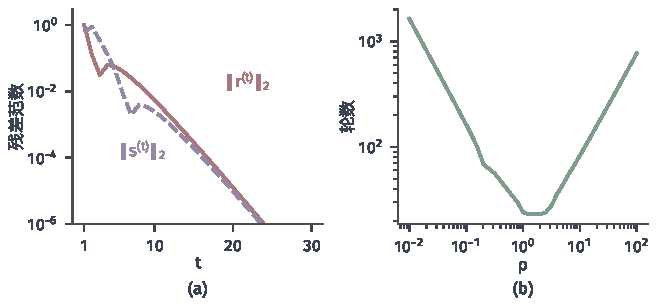
\includegraphics[width=112mm]{figures/05-optimization/06-constrained-optimization/matplotlib/pm-admm-lasso/figure.pdf}
  \caption{小例子上的ADMM。(a)半对数坐标，$\rho=1$，红线是原始残差，紫色虚线是对偶残差。(b)双对数坐标，两个残差都小于$10^{-6}$所需的轮数随$\rho$的变化。两端都慢，中间有一段较宽的平坦区域。}
  \label{fig:pm-admm-lasso}
\end{BookInlineFigure}

\subsection{收敛与实现}
\label{sec:pm-admm-convergence}

\paragraph{收敛定理}
ADMM的步子不是ALM的精确子问题，上一节的定理不能直接用，需要一个专门的证明。证明的想法是构造一个Lyapunov函数，它把乘子误差和$\bm{z}$的误差放在一起，每一轮都下降。

\begin{theorem}[两块ADMM的收敛]
\label{thm:pm-admm-convergence}
设$f,g$是适当、闭的凸函数，固定$\rho>0$，式~\eqref{eq:pm-admm}的两个子问题的最小点存在并精确求解。设$\mathcal{L}_0$有鞍点$(\bm{x}^\star,\bm{z}^\star,\bm{\nu}^\star)$，记$p^\star=f(\bm{x}^\star)+g(\bm{z}^\star)$，$p^{(t)}=f(\bm{x}^{(t)})+g(\bm{z}^{(t)})$，并记
\begin{equation}
 V^{(t)}=\frac1\rho\lVert\bm{\nu}^{(t)}-\bm{\nu}^\star\rVert_2^2+\rho\lVert\bm{B}(\bm{z}^{(t)}-\bm{z}^\star)\rVert_2^2 .
 \label{eq:pm-admm-lyapunov}
\end{equation}
则$t\geq1$时
\begin{equation}
 V^{(t+1)}\leq V^{(t)}-\rho\lVert\bm{r}^{(t+1)}\rVert_2^2-\rho\lVert\bm{B}(\bm{z}^{(t+1)}-\bm{z}^{(t)})\rVert_2^2 ,
 \label{eq:pm-admm-descent}
\end{equation}
并且$\bm{r}^{(t)}\to\bm{0}$，$\bm{s}^{(t)}\to\bm{0}$，$p^{(t)}\to p^\star$。若$\bm{A},\bm{B}$还列满秩，则$\bm{x}^{(t)},\bm{z}^{(t)},\bm{\nu}^{(t)}$都收敛，其极限构成一个鞍点。
\end{theorem}

\begin{proof}
记$\bm{r}=\bm{r}^{(t+1)}$，$\bm{w}=\bm{B}(\bm{z}^{(t+1)}-\bm{z}^{(t)})$。证明分四步。

第一步，用鞍点给出一侧不等式。鞍点满足
\[
 \mathcal{L}_0(\bm{x}^\star,\bm{z}^\star,\bm{\nu}^\star)\leq\mathcal{L}_0(\bm{x}^{(t+1)},\bm{z}^{(t+1)},\bm{\nu}^\star),
\]
再用$\bm{A}\bm{x}^\star+\bm{B}\bm{z}^\star=\bm{c}$，于是
\begin{equation}
 p^\star-p^{(t+1)}\leq\langle\bm{\nu}^\star,\bm{r}\rangle .
 \label{eq:pm-admm-proof-a}
\end{equation}

第二步，用子问题的最优性给出另一侧不等式。上一小节已经推导，$\bm{x}^{(t+1)}$最小化凸函数$f(\bm{x})+\langle\bm{\nu}^{(t+1)}-\rho\bm{w},\bm{A}\bm{x}\rangle$，$\bm{z}^{(t+1)}$最小化凸函数$g(\bm{z})+\langle\bm{\nu}^{(t+1)},\bm{B}\bm{z}\rangle$。分别在$\bm{x}^\star$、$\bm{z}^\star$处比较，得到
\[
 f(\bm{x}^{(t+1)})+\langle\bm{\nu}^{(t+1)}-\rho\bm{w},\bm{A}\bm{x}^{(t+1)}\rangle\leq f(\bm{x}^\star)+\langle\bm{\nu}^{(t+1)}-\rho\bm{w},\bm{A}\bm{x}^\star\rangle,
\]
\[
 g(\bm{z}^{(t+1)})+\langle\bm{\nu}^{(t+1)},\bm{B}\bm{z}^{(t+1)}\rangle\leq g(\bm{z}^\star)+\langle\bm{\nu}^{(t+1)},\bm{B}\bm{z}^\star\rangle .
\]
两式相加。由$\bm{A}\bm{x}^\star+\bm{B}\bm{z}^\star=\bm{c}$，有
\[
 \bm{A}(\bm{x}^{(t+1)}-\bm{x}^\star)+\bm{B}(\bm{z}^{(t+1)}-\bm{z}^\star)=\bm{r},
\]
所以含$\bm{\nu}^{(t+1)}$的项合并成$\langle\bm{\nu}^{(t+1)},\bm{r}\rangle$。再把$\bm{A}(\bm{x}^{(t+1)}-\bm{x}^\star)$换成$\bm{r}-\bm{B}(\bm{z}^{(t+1)}-\bm{z}^\star)$，得到
\begin{equation}
 p^{(t+1)}-p^\star\leq-\langle\bm{\nu}^{(t+1)},\bm{r}\rangle+\rho\langle\bm{w},\bm{r}-\bm{B}(\bm{z}^{(t+1)}-\bm{z}^\star)\rangle .
 \label{eq:pm-admm-proof-b}
\end{equation}

第三步，推导下降不等式。式~\eqref{eq:pm-admm-proof-a}与式~\eqref{eq:pm-admm-proof-b}相加，左边为零，两边乘$2$并移项，得到
\[
 2\langle\bm{\nu}^{(t+1)}-\bm{\nu}^\star,\bm{r}\rangle-2\rho\langle\bm{w},\bm{r}\rangle+2\rho\langle\bm{w},\bm{B}(\bm{z}^{(t+1)}-\bm{z}^\star)\rangle\leq0 .
\]

第一项用$\bm{\nu}^{(t+1)}=\bm{\nu}^{(t)}+\rho\bm{r}$改写，按乘子距离的平方差展开：
\[
 2\langle\bm{\nu}^{(t+1)}-\bm{\nu}^\star,\bm{r}\rangle
 =\frac1\rho\Bigl(\lVert\bm{\nu}^{(t+1)}-\bm{\nu}^\star\rVert_2^2-\lVert\bm{\nu}^{(t)}-\bm{\nu}^\star\rVert_2^2\Bigr)+\rho\lVert\bm{r}\rVert_2^2 .
\]
第三项要用下面的恒等式：
\[
 2\langle\bm{a}-\bm{b},\bm{a}\rangle=\lVert\bm{a}\rVert_2^2-\lVert\bm{b}\rVert_2^2+\lVert\bm{a}-\bm{b}\rVert_2^2 .
\]
取$\bm{a}=\bm{B}(\bm{z}^{(t+1)}-\bm{z}^\star)$，$\bm{b}=\bm{B}(\bm{z}^{(t)}-\bm{z}^\star)$，此时$\bm{a}-\bm{b}=\bm{w}$，于是
\[
 2\rho\langle\bm{w},\bm{a}\rangle=\rho\lVert\bm{a}\rVert_2^2-\rho\lVert\bm{b}\rVert_2^2+\rho\lVert\bm{w}\rVert_2^2 .
\]
把这两式代回，合并成
\[
 V^{(t+1)}-V^{(t)}+\rho\lVert\bm{r}\rVert_2^2+\rho\lVert\bm{w}\rVert_2^2-2\rho\langle\bm{w},\bm{r}\rangle\leq0 .
\]

只差$\langle\bm{w},\bm{r}\rangle$的符号。设$t\geq1$，$\bm{z}^{(t)}$也是上一轮的子问题解，最小化$g(\bm{z})+\langle\bm{\nu}^{(t)},\bm{B}\bm{z}\rangle$。把它和$\bm{z}^{(t+1)}$的最优性互相比较，
\[
 g(\bm{z}^{(t+1)})+\langle\bm{\nu}^{(t+1)},\bm{B}\bm{z}^{(t+1)}\rangle\leq g(\bm{z}^{(t)})+\langle\bm{\nu}^{(t+1)},\bm{B}\bm{z}^{(t)}\rangle,
\]
\[
 g(\bm{z}^{(t)})+\langle\bm{\nu}^{(t)},\bm{B}\bm{z}^{(t)}\rangle\leq g(\bm{z}^{(t+1)})+\langle\bm{\nu}^{(t)},\bm{B}\bm{z}^{(t+1)}\rangle .
\]
相加后，$g$的项全部消去，剩下
\[
 \langle\bm{\nu}^{(t+1)}-\bm{\nu}^{(t)},\bm{w}\rangle\leq0 ,
\]
也就是$\rho\langle\bm{r},\bm{w}\rangle\leq0$。于是$-2\rho\langle\bm{w},\bm{r}\rangle\geq0$，舍去后即得式~\eqref{eq:pm-admm-descent}。

第四步，取极限。对式~\eqref{eq:pm-admm-descent}求和，$\sum_t\lVert\bm{r}^{(t)}\rVert_2^2$和$\sum_t\lVert\bm{w}\rVert_2^2$都有限，所以$\bm{r}^{(t)}\to\bm{0}$，$\bm{B}(\bm{z}^{(t+1)}-\bm{z}^{(t)})\to\bm{0}$，进而$\bm{s}^{(t)}\to\bm{0}$。同时$V^{(t)}$有界，所以$\bm{\nu}^{(t)}$和$\bm{B}\bm{z}^{(t)}$都有界。式~\eqref{eq:pm-admm-proof-b}的右边因此趋于零，式~\eqref{eq:pm-admm-proof-a}的右边也趋于零，夹逼得$p^{(t)}\to p^\star$。

最后设$\bm{A},\bm{B}$列满秩。$\bm{B}\bm{z}^{(t)}$有界推出$\bm{z}^{(t)}$有界，再由$\bm{r}^{(t)}\to\bm{0}$推出$\bm{A}\bm{x}^{(t)}$有界，从而$\bm{x}^{(t)}$有界。

取一个收敛子列，极限记为$(\hat{\bm{x}},\hat{\bm{z}},\hat{\bm{\nu}})$。在$\bm{r}=\bm{0}$、最优性包含式~\eqref{eq:pm-admm-x-optimality}和$\bm{z}$的最优性条件里取极限（闭凸函数的次微分图像是闭的），可知极限满足KKT条件~\eqref{eq:pm-admm-kkt}，所以它是鞍点。

式~\eqref{eq:pm-admm-descent}对任意鞍点成立。取这个鞍点作为比较点，$V^{(t)}$单调不增且沿子列趋于零，所以整列趋于零。再由列满秩，$\bm{x}^{(t)},\bm{z}^{(t)},\bm{\nu}^{(t)}$整列收敛。
\end{proof}

定理的各部分有不同的强度。残差和目标值的收敛只需要鞍点存在。在没有列满秩的一般情形下，$\bm{\nu}^{(t)}$本身也收敛到某个最优乘子，这个结论可以从ADMM与Douglas--Rachford分裂的等价关系得到，证明需要算子分裂的不动点理论，篇幅较长，这里只使用结论。

原始变量的整列收敛则确实需要额外条件。$\bm{A}$不是列满秩时，$\bm{x}$可以在$\operatorname{null}(\bm{A})$方向上不确定，子问题的解都不唯一，序列没有理由收敛。

\paragraph{实现中的计算}
ADMM每轮的代价取决于两个子问题。套索的例子中，$\bm{x}$更新要解以$\bm{D}^\top\bm{D}+\rho\bm{I}$为系数的线性系统，$\rho$固定时这个矩阵只需分解一次。一次Cholesky分解约需$O(n^3)$次运算，此后每轮只需$O(n^2)$次前代和回代。

当$N\ll n$时，用矩阵求逆引理转化为$N\times N$的系统，分解成本降为$O(N^2n)$。$\bm{z}$更新是逐坐标的软阈值，只需$O(n)$。

分布式的场合，$\bm{x}$和$\bm{z}$常放在不同机器上，每轮通信量是一个残差大小的向量。与联合求解的ALM比较，ADMM的单轮代价低，通信轮数多。ADMM的典型行为是前面几十轮到达中等精度，此后缓慢收敛，所以适合中等精度的问题。

\paragraph{子问题的精度}
定理要求子问题精确求解。实际上线性系统用迭代法解，或者子问题本身没有闭式解。凸的情形下，只要各轮的误差可和，收敛结论仍然成立，证明需要把误差项带入上述下降不等式，并做累加估计。内层精度不够时，$\bm{x}$的最优性条件~\eqref{eq:pm-admm-x-optimality}有一个误差项，所以对偶残差$\bm{s}$不再完全反映驻定误差，需要另外监控子问题的残差。

\paragraph{多块与非凸}
从形式上看，把两块推广到三块只是多写一行，但保证不能沿用。有一个三块的反例：
\[
 \min\ 0\qquad\text{s.t.}\qquad\bm{a}_1x_1+\bm{a}_2x_2+\bm{a}_3x_3=\bm{0},
\]
其中$\bm{a}_1=(1,1,1)$，$\bm{a}_2=(1,1,2)$，$\bm{a}_3=(1,2,2)$。系数矩阵可逆，唯一解是原点，目标是常数$0$。按三块逐块更新，$\rho=1$。数值计算给出这个线性迭代矩阵的谱半径约为$1.028>1$，所以序列从几乎任何初值出发都发散。

图~\ref{fig:pm-admm-threeblock}中，红线是三块更新的残差，一直增长；绿线把后两块合并成一块，按两块ADMM更新，残差下降。这个例子的目标恒为零，每个子问题都精确可解，失败的原因只在更新的结构上。

\begin{BookInlineFigure}
  \centering
  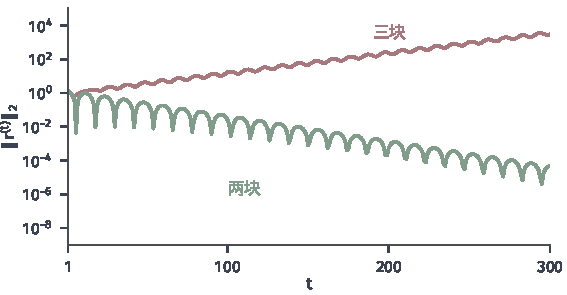
\includegraphics[width=96mm]{figures/05-optimization/06-constrained-optimization/matplotlib/pm-admm-threeblock/figure.pdf}
  \caption{同一个线性系统上的三块与两块ADMM，$\rho=1$，半对数坐标，初值$\bm{x}^{(0)}=(1,1,1)$，乘子初值为零。红线是逐块更新三块的残差，发散；绿线把后两块合并成一块，收敛。}
  \label{fig:pm-admm-threeblock}
\end{BookInlineFigure}

非凸问题上的ADMM使用很广，但一般只能保证在额外的结构条件下收敛到驻点，有时需要$\rho$足够大，有时根本不收敛。一个非凸改写在形式上和ADMM相同，并不意味着上面的定理适用，每种情形都需要重新分析。结束时仍然要回到原约束和最优性条件上去检查。

\section{方法比较与计算成本}
\label{sec:pm-comparison}

本节回答一个实际问题：同一个约束问题，四种方法到底哪里不同，比较代价时应该数什么。

\paragraph{各方法改变了什么}
四种方法都在做同一件事，把约束的信息换成原始变量子问题里的一项。它们的差别可以按三个方面读出来：给目标加了什么，乘子怎样更新，原始变量怎样求解。

\begin{BookInlineTable}
  \centering
  \small
  \begin{tabular}{@{}llll@{}}
    \toprule
    方法 & 目标的改动 & 乘子 & 原始变量\\
    \midrule
    二次罚 & 加平方罚 & 无（$\rho h$仅作估计） & 逐轮全部求解\\
    一次罚 & 加一次罚 & 无（门槛内隐含） & 非光滑子问题\\
    对偶上升 & 加线性价格 & 显式步 & 可分块，全部求解\\
    ALM & 价格加平方罚 & 隐式步，步长$\rho$ & 联合求解\\
    ADMM & 价格加平方罚 & 步长$\rho$ & 两块各更新一次\\
    \bottomrule
  \end{tabular}
  \caption{各方法的结构对照。}
  \label{tab:pm-structure}
\end{BookInlineTable}

\paragraph{相同精度下的代价}
比较时要固定口径。各方法的罚目标函数不同，比较目标值没有意义；ADMM的一轮和ALM的一轮完成的工作也不同，比较轮数同样没有意义。合理的办法是固定同一个问题，要求达到相同的原始精度，再分别统计外层轮数、内层计算和通信。

下面用二元例，都从原点出发，要求$\lvert h(\bm{x})\rvert\leq10^{-3}$。内层的梯度法取步长$1/L$，容差为$10^{-6}$，这样内层误差不干扰外层。ADMM的两个子问题都是一元二次函数的最小化，取闭式解。

\begin{BookInlineTable}
  \centering
  \small
  \begin{tabular}{@{}lrrrr@{}}
    \toprule
    方法 & 外层轮数 & 内层梯度步 & 矩阵分解 & 最大条件数\\
    \midrule
    二次罚（$\rho$乘$10$） & $5$ & $123443$ & $5$ & $15001$\\
    对偶上升（$\alpha=0.6$） & $7$ & $162$ & $0$ & $3$\\
    ALM（$\rho=1.5$） & $8$ & $230$ & $1$ & $3.1$\\
    ADMM（$\rho=1.5$） & $11$ & 闭式 & $0$ & 无\\
    \bottomrule
  \end{tabular}
  \caption{二元例中达到$\lvert h\rvert\leq10^{-3}$的代价。“矩阵分解”指改用直接法解内层时需要的分解次数。这些数字只对这个例子有效。}
  \label{tab:pm-cost}
\end{BookInlineTable}

表~\ref{tab:pm-cost}和图~\ref{fig:pm-compare}说明了几件事。二次罚外层轮数最少，内层步数却多出几个数量级，几乎全部花在最后两轮的病态问题上。ALM比二次罚多几轮，却始终在解同一个良态问题。

对偶上升在这里表现很好，因为$f$是强凸的，内层矩阵的条件数只有$3$，步长也事先选好了。如果把目标改成线性的，或者步长取到$1.5$，它就失效了，表中的数字不能外推。ADMM在这里每个子问题都是一元的，所以一轮很便宜，但一轮要交换一次信息。在通信比本地计算贵得多的环境中，轮数才是主要成本。

\begin{BookInlineFigure}
  \centering
  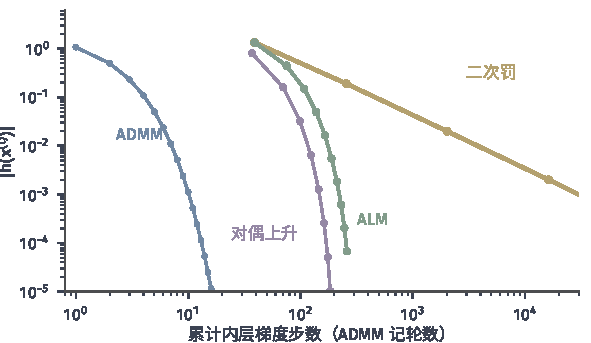
\includegraphics[width=100mm]{figures/05-optimization/06-constrained-optimization/matplotlib/pm-compare/figure.pdf}
  \caption{二元例上约束残差随累计计算量的下降，双对数坐标。黄线是二次罚，紫线是对偶上升，绿线是ALM，横轴是累计的梯度步数（内层容差$10^{-6}$）；蓝线是ADMM，横轴是轮数，两者的单位不同，只宜比较曲线的走势。}
  \label{fig:pm-compare}
\end{BookInlineFigure}

\paragraph{比较时容易出错的地方}
第一，不同方法的罚目标值不可比。$Q_\rho$、$E_\rho$、$\mathcal{L}_\rho$的数值里都混有罚项，要比较的是原目标和约束违规，或者驻定残差。

第二，只比较一次内层更新的速度会误导。一次梯度步的时间四种方法差不多，但需要多少步完全取决于子问题的条件数；对偶上升的内层便宜，可能需要更多外层轮数。

第三，精度要对等。一个方法返回约束残差$10^{-3}$的点，另一个返回$10^{-6}$的点，前者的目标值可能因为更不可行而显得更低。

第四，不同方法适用的问题不同，这个例子凸、光滑、约束线性。约束非线性时，对偶上升和ADMM的结论都要重新检查；目标非凸时，ALM的局部结论才是相关的。选择方法时应先看问题的结构：约束少而目标规模大时考虑ALM，目标和约束可分时考虑对偶分解或ADMM，只需要中等精度且子问题便宜时考虑ADMM，需要高精度时考虑ALM或者后面两章的方法。

\section{本章小结}
\label{sec:pm-summary}

本章从一个问题开始：允许迭代点暂时违反约束，用什么信号把它拉回来。

惩罚方法给违规计价。二次罚光滑，但边界上没有回推的力，有限的$\rho$总留下违规，$\rho\to\infty$时法向曲率随之增长，子问题越来越病态。一次罚在边界上有尖角，$\rho$超过最优乘子的最大绝对分量后最小点就是原问题的解，代价是目标不可微。“精确”的含义是解的对应，全局结论需要强对偶和对偶解存在，局部结论需要误差界或二阶条件。

对偶上升直接调整价格。解完Lagrange子问题，约束残差就是对偶函数的超梯度，目标可分时各块可以独立求解。它改进的是下界，迭代点通常不可行，步长受限，$q$不可微时单步未必上升；要得到原始解，需要平均、选解或修复，并且同时报告可行性和间隙。

增广Lagrange法把价格和平方罚合在一起。乘子提供大部分的力，罚项修正余下的部分，所以有限的$\rho$就够了。从对偶问题看，它是隐式的邻近点步，比显式的对偶上升稳定得多，凸问题中任何固定的$\rho>0$都收敛。代价是平方项把变量耦合起来，子问题更难。不等式要用正部形式，乘子要保持非负。

ADMM把两块变量各更新一次，用一次乘子更新代替联合求解。这样既保留乘子的稳定性，又能分别利用两块结构，代价是出现了对偶残差。原始残差和对偶残差要一起看，$\rho$改变时缩放乘子要同步换算。两块闭凸目标在鞍点存在时有收敛保证，多块或非凸的情形不能沿用。

\begin{BookInlineTable}
  \centering
  \small
  \begin{tabular}{@{}lll@{}}
    \toprule
    方法 & 主要条件 & 能保证什么\\
    \midrule
    二次罚 & 各轮全局解，$\rho\to\infty$ & 聚点全局最优\\
    一次罚 & 强对偶，$\rho$超过门槛 & 最小点集合相同\\
    对偶上升 & 残差来自全局最小点 & 超梯度；凸时平均点渐近可行\\
    ALM & 凸，强对偶，固定$\rho$ & 残差趋零，目标值收敛\\
    ADMM & 两块闭凸，鞍点存在 & 两种残差趋零，目标值收敛\\
    \bottomrule
  \end{tabular}
  \caption{本章各方法的主要条件与保证。局部结论和近似求解下的结论见各节。}
  \label{tab:pm-summary}
\end{BookInlineTable}

几种方法结束时要做的事是一样的：回到原约束检查可行性，回到Lagrange函数检查驻定，有不等式时检查互补；需要全局结论时，再用对偶值或者凸性给出证书。第~\ref{chap:sequential-quadratic-programming}章接着处理光滑非线性约束，用局部二次模型同时更新原始变量和乘子。

